\documentclass[
  12pt,
  a4paper,
  parskip,
  openany
]{scrbook}

\usepackage{scrhack}
\usepackage[utf8]{inputenc}
\usepackage[english]{babel}

\usepackage[hidelinks, pdfpagelabels, pdfusetitle]{hyperref}
\hypersetup{hypertexnames=false}
\usepackage{enumitem}
\usepackage{suffix}
\usepackage{lipsum}
\usepackage{tabularx}
\usepackage{graphicx}
\usepackage{float}
\usepackage[title,titletoc,header,toc,page]{appendix}
\renewcommand{\appendixname}{Appendix}

% Layout refinements
% Also fixes overfull hbox due to texttt
\usepackage{microtype}

% Abbreviations
\usepackage{glossaries-extra}
\setabbreviationstyle{long-short}
\setabbreviationstyle[acronym]{long-short}
\makeglossaries
\newacronym{sql}{SQL}{Structured Query Language}
\newacronym{cql}{CQL}{Cassandra Query Language}
\newglossaryentry{nosql}{
  name={NoSQL},
  description={
    \textit{No SQL} or \textit{Not only SQL}.
    NoSQL is a loosely defined term, grouping different
    databases which either do not only support data
    accesses via the Structured Query Language (SQL),
    or do not support it at all.
  },
}

\newglossaryentry{jpeg}{
  name={JPEG},
  description={
    Method for compression of image data developed by the \textit{Joint Photographic Experts Group}.
  },
}

\newglossaryentry{cap}{
  name={CAP theorem},
  description={
    The CAP theorem (also called Brewer's theorem) states, that in a
    distributed database system, it is not possible to achieve more than
    two characteristics out of \textit{consistency}, \textit{availability}
    and \textit{partition tolerance} \cite{brewer2000}.
  },
}

\newacronym{crud}{CRUD}{Create, Read, Update, Delete}
\newacronym{it}{IT}{information technology}
\newacronym{orm}{ORM}{object-relational mapping}
\newacronym{rdbms}{RDBMS}{relational database management system}
\newacronym{dbms}{DBMS}{database management system}
\newacronym{oltp}{OLTP}{online transaction processing}
\newacronym{http}{HTTP}{HyperText Transfer Protocol}
\newacronym{tcp}{TCP}{transmission control protocol}
\newacronym{bsd}{BSD}{Berkeley Software Distribution}
\newacronym{resp}{RESP}{Redis serialization protocol}
\newacronym{ram}{RAM}{random access memory}
\newacronym{ssd}{SSD}{solid state drive}
\newacronym{sata}{SATA}{serial ATA}
\newacronym{cpu}{CPU}{central processing unit}
\newacronym{iommu}{IOMMU}{input/output memory management unit}
\newacronym{ddr4}{DDR4}{double data rate 4}
\newacronym{hdd}{HDD}{hard disk drive}
\newacronym{ecc}{ECC}{error correcting code}
\newacronym{ascii}{ASCII}{American Standard Code for Information Interchange}
\newacronym{btrfs}{BTRFS}{Better File System (modern copy on write filesystem)}
\newacronym{api}{API}{application programming interface}
\newacronym{mdm}{MDM}{master data management}
\newacronym{ogm}{OGM}{object-graph mapping}
\newacronym{iam}{IAM}{identity and access management}
\newacronym{acid}{ACID}{atomicity, consistency, isolation, durability}

\newglossaryentry{cern}{
  name={CERN},
  description={
    CERN, the European Organization for Nuclear Research, is one of the world's
    largest and most respected centres for scientific research.
  },
}
\newglossaryentry{atlas}{
  name={ATLAS},
  description={
   ATLAS (A Toroidal LHC ApparatuS) is one of the seven particle detector
   experiments at the Large Hadron Collider (LHC), a particle accelerator at CERN.
   It generates 1 petabyte of raw data per second, even after filtering it
   still requires over 100 megabytes of disk space per second – at least a
   petabyte each year \autocite{fermi2004giant}.
  },
}


% Listings and drawings (needs to be loaded before csquotes)
\usepackage{minted}
\usemintedstyle[js]{vs}
\usepackage{tikz}
\usetikzlibrary{intersections,arrows.meta}


% Citation packages and options
\usepackage{csquotes}
\usepackage[
  backend=biber,
  style=apa,
]{biblatex}
\addbibresource{bibliography.bib}
% Break long URLs in sources
\setcounter{biburllcpenalty}{7000}
\setcounter{biburlucpenalty}{8000}

\DeclareLanguageMapping{english}{english-apa}


% Correct listing references
\providecommand*{\listingautorefname}{Listing}

% ===== INDIVIDUAL AUTHORS PER CHAPTER =====
% Source: https://tex.stackexchange.com/a/156865
\newcommand\chapterauthor[1]{\authortoc{#1}\printchapterauthor{#1}}
\WithSuffix\newcommand\chapterauthor*[1]{\printchapterauthor{#1}}

\makeatletter
\newcommand{\printchapterauthor}[1]{%
  {\parindent0pt\vspace*{-25pt}%
  \linespread{1.1}\large#1%
  \par\nobreak\vspace*{35pt}}
  \@afterheading%
}
\newcommand{\authortoc}[1]{%
  \addtocontents{toc}{\vskip-10pt}%
  \addtocontents{toc}{%
    \protect\contentsline{chapter}%
    {\hskip1.3em\mdseries\protect\scriptsize#1}{}{}}
  \addtocontents{toc}{\vskip5pt}%
}
\makeatother
% ==========================================


\title{NoSQL Databases}
\author{Course STG-TINF16A of the Baden-Wuerttemberg\\ Cooperative State University Stuttgart}
\date{\today}

\begin{document}

\maketitle
\tableofcontents


\printglossaries

\chapter{Introduction}

In a world of unstructured data, \gls{nosql} Databases are of never-ending
popularity.  While \acrshort{sql} databases are still the most popular, two out
of the ten most used databases already are \gls{nosql}
\parencite{dbenginesRanking}.  The trends show that the interest in \gls{nosql}
increases a lot faster than in traditional databases \parencite[section
\texttt{ranking\_categories}]{dbenginesRanking}. That shows that it is
necessary to consider \gls{nosql} databases as alternatives for relational
databases and to discuss their advantages as well as their disadvantages.

The hype around \gls{nosql} Databases in today's landscape can not be
disregarded.  The popularity for \gls{nosql} databases has been steadily
increasing and gaining fans from all over the database community.

But the term \gls{nosql} was first used in 1998 already, introduced by Carlo
Strozzi. While the term can mean either 'not only SQL' or 'no SQL', it is
uniform in the meaning of not being a relational database system. Soon after,
in the beginning of the next century, \gls{nosql} really started gaining
momentum and first implementations of different technologies started coming up.
One of the first \gls{nosql} technologies to come up was the document oriented
database implementation Metakit, soon followed by the first ever graph database
Neo4j in the year 2000. After that, many more followed and \gls{nosql}
databases have become a central point to the database landscape today. 

While it is clear that \gls{nosql} databases will not replace all other
\glspl{dbms} in existence today, they are especially popular in a few distinct
scenarios: For instance, when prototyping a new application while the data
format is still undecided, \gls{nosql} databases provide developers with
flexibility unseen in usual relational \glspl{dbms}. In addition to that, the
fast response and processing times can drastically increase an application's
performance, if used correctly. Also, the ability to store data which does not
adhere to a constant schema is significant with ever-changing and
uncontrollable data sources.

With the increasing amount of databases offered, choosing the right one can be
overwhelming. Not only does one need to decide for the right data structure,
but also find an implementation that fits the needs of your application.

Due to this growing importance of NoSQL databases in today's IT-landscape and
the abundance of different technologies implementing NoSQL, it is of great
importance to provide some guidance for this topic. For this reason this book
delivers not only an overview over some of the most popular NoSQL databases but
also analyses their features in the context of the CAP-theorem developed by
Brewer.

This eBook gives an overview of different types of \gls{nosql} technologies
that are relevant today. First, it will talk about Key-Value databases
including a quick general introduction and the selected implementations
Hazelcast, Redis and Riak. After that, Column Wide Oriented databases are
introduced, including the basics of Cassandra. Chapter 4 focuses on Documented
Oriented databases like Couchbase and Rethink DB. Lastly, the principals of
Graph databases are described with Neo4j as an example implementation. 




\chapter{Key-value databases}
\chapterauthor{Vanessa Jörns, Tobias Schiffmann and Victor Veal}
Key-value databases or key-value stores are a classification of NoSQL databases. 
The idea of key-value stores is to collect a key  for every data set. Each set that is stored in the database can be accessed by the key. Therefore the key needs to be distinct, whether in a namespace or in the whole system. The database system has no pattern for the values which is why it is not  necessary to know about the type of the values that are stored. This feature enables easy storage of any kind of data like serialized structures, XML, text data, files...  \parencite{keyValueIntro}.


However, there are also disadvantages of this database management type. In terms of operational actions like querying through the data, as one would do in relational database management systems, key-value databases only provide simple operations like get, put and delete. As a result of this constraint, data querying must be handled at the application level. 

Another difference to relational databases are the use cases. 
 For simple applications, which only require a system that is able to store and manage data (e.g. update entries, join tables), is capable of representing real-world entities and describes relationships, relational databases should be used. Key-value databases should rather be chosen if the application or the system requires a good performance since key-value solutions are faster than relational database systems \parencite{keyValueUsecase}.
 
For instance, an online application that is only responsible to enable quick access to a profile, does not need to interact with entries of the profile itself. It should rather guarantee that the user of the application can easily find the profile by providing the corresponding key. To enable a quick access of the profile, it would be enough to only search for the unique ID of the profile instead of querying across several attributes of the data set.

Nevertheless, not all key-value solutions are similar designed. There are a lot of different systems today. In the following chapters some database management systems will be introduced. The focus will be on providing the reader a quick overview about the different systems, how they distinguish from each other and how to use them.

The first system that will be explained is Hazelcast which gives an overview of the the basic characteristics including a cheat sheet with needed commands. The next section talks about Redis and the basic features as well as in-memory computing. Last but not least the Key Value chapter is finished with a section about Riak. 


% eventuell Bild
% [1] https://en.wikipedia.org/wiki/Key-value_database#/media/File:KeyValue.PNG

\section{Hazelcast}
\chapterauthor{Vanessa Jörns, Tobias Schiffmann and Victor Veal}

\subsection{Introduction}

Hazelcast is a company that is developing an in-memory computing platform consisting of Hazelcast IMDG, Hazelcast Jet and Hazelcast Cloud. “Hazelcast Jet is an embeddable, distributed computing platform for fast processing of big data sets”. It is built on the foundation of Hazelcast IMDG on which this chapter focuses \parencite{hazelcast}.

An in-memory data grid (IMDG) is a rather new concept where data is stored in the main memories of a computing cluster. One of the main aspects is the ability to automatically scale and rebalance the cluster when decreasing or increasing in size. Here the data is partitioned equally across the cluster nodes. IMDGs are usually used for implementing distributed and scalable applications since they provide distributed versions of the basic data structures \parencite{tasci2015}. Hazelcast IMDG is open source and implemented in Java. However, there are also existing API’s for C/C++, .NET, REST, Python, Go and Node.js.

As Hazelcast is designed to be lightweight and easy to use, it can be downloaded as a compact library (JAR) and can be used by simply adding this JAR file to the classpath. With Java as the only dependency there is no need to install any software \parencite{hazelcastmanual}.

Firstly, the features of Hazelcast are specified and distinguished from other key-value solutions. The next section talks about the CAP theorem and how it applies to Hazelcast. After that a short manual for implementing Hazelcast for own applications is provided. This inlcudes a basic set up as well as a configuration. For reference a cheat sheet with the most important commands is included. In the end, the whole chapter about Hazelcast is concluded and the advantages and disadvantages are analyzed. 
\subsection{Specification}
Hazelcast consists of many same or similar features like other key value databases and IMDGs. However, there are some major features which describe Hazelcast’s distinctive strengths.
The first and one of the main characteristics is that Hazelcast completely computes in-memory rather than storage based.  This makes Hazelcast extremely fast but also volatile.

Another major feature is that Hazelcast relies on clustering with the approach of a “masterless nature” of the nodes. This means that each node in the cluster has the exact same functionality and operates in a peer-to-peer manner \parencite{johns2015}. So unlikely other NoSQL databases, there is no master and slave hence there is no single point of failure. All nodes are responsible for the same proportion of processing and storing \parencite{hazelcastmanual}. The oldest node of the cluster automatically becomes the “de facto leader” and manages the distribution of the data for joining nodes. Since the data is redistributed for every joining or exiting node, the cluster rebalances automatically and thus makes Hazelcast simple to set up and configure.

As Hazelcast consists of the basic features of an in-memory data grid, the data and therefore the load is equally spread across the cluster. Here each node is the owner and holds a number of partitions of the overall data.
Therefore, saturation of a cluster can simply be overcome by adding more nodes to the cluster. The cluster is then rebalanced and the load for each node decreases. This means scaling is easy and fast which makes Hazelcast suitable for handling big amounts of data.
Nevertheless, since Hazelcast persists data entirely in-memory, it has the main drawback that data will be lost with a node shutting down. To prevent the overall cluster of losing the data a failing node has held, Hazelcast distributes backups of each data partition among multiple other members. This means in case of a node shut down, another node will have a backup of the data and the cluster can be rebalanced without suffering any data loss and downtime \parencite{johns2015}.
\begin{figure}[H]
    \centering
    \includegraphics[scale=0.6]{img/hazelcast-nodes.png}
    \caption{Hazelcast Nodes \parencite{johns2015}}
\end{figure}
This illustration shows the cluster structure as described above. It explains how the data is partitioned in equal parts and spread across the cluster as well as the replication of the data for backup. This is just a simplified version of the structure with only three nodes. In practice each node would be responsible for multiple subsets of the data and not just one data partition. So, for instance in order to get the data of Partition 1, the application has to communicate with Node 1. The distribution of the data is dynamic and which node is responsible for which subset of data usually changes over time. Hence, the allocation is an internal operational detail and the application as well as the user usually does not need to know it.
Moreover, Hazelcast supports various distributed collectors, features and processors. Besides storing the data in-memory distributed on many nodes, it is possible to load data from diverse sources into varying structures, communicate across the cluster by sending messages and to use the stored data for analytical processing \parencite{johns2015}.


\subsection{Hazelcast and the CAP theorem}
As Hazelcast enables data storage for distributed systems, it may be interesting how the CAP theorem applies to it. According to the chapters before, Hazelcast offers a storage mechanism that distributes data across several nodes. Therefore the first aspect out of the CAP theorem is network partitioning. According to the article \textit{Jepsen Analysis on Hazelcast 3.8.3} \parencite{hazelcastCP}, Hazelcast is a PA system which means that it favours availability over consistency. Due to the fact that data is partitioned, the problem of keeping the data consistent over the whole system occurs. For example, if the user inserts a new entry to a cluster, the whole systems needs to update this info so that the same information can be provided from all nodes. This problem of having several nodes storing inconsistent data is called split brain in an In-Memory Data Grid system.

Hazelcast offers a method that should avoid split brain. In the so called "Split Brain Protection" a minimum number of nodes is set on which write or read operations are prevented. If a split brain happens, any sub-clusters that have a lower number of nodes than the minimum number are prevented from accepting write operations. Nevertheless, this method only reduces the time of inconsistency. Therefore it does not completely avoid the inconsistent state of the system \parencite{hazelcastCP}.

Recently, the Hazelcast company has announced the ability to provide a solution that supports both PA (availability over consistency) and PC (constistency over availability). This feature should allow the user to adapt more flexibly to the requirements of the application. So far, there are too less resources that can describe this new feature of Hazelcast which is why this paper is currently not able to report about it \parencite{hazelcastCAP}.

\subsection{Implementation}
\subsubsection*{Getting Started}
As already mentioned Hazelcast is designed to be easy to use and therefore only require a few steps to set it up running.
First of all, the Hazelcast package has to be downloaded, for example from the official website \parencite{hazelcast:hazelcastDownload}. The package is offered in a compressed data format and has to be extracted afterwards.

Hazelcast does not need any software installations. It is written in Java and therefore the platform to run Hazelcast on needs to be able to execute Java code. To do so a Java Development Kit has to be ready to use which can be gathered from the Oracle website. After ensuring Java code to run, Hazelcast is ready to be used.

The console application is an easy way to get in touch with Hazelcast and experience the software. It can be started by executing the \texttt{console} scripts in the \texttt{demo/} directory from a terminal. Hazelcast creates a new member which will either create a new cluster or will join a cluster if there already exists one. The cluster can than be filled by typing the commands as the following example shows.
\begin{flushleft}
\begin{figure}[h]
    \includegraphics{img/hazelcastPut.PNG} 
    \caption{Hazelcast Basic Commands \parencite{johns2015}}
\end{figure}
\end{flushleft}
When executing the scripts in another window, Hazelcast shows how the new member joins the cluster and displays the two members and there addresses after a short period of time.

\begin{flushleft}
\begin{figure}[h]
    \includegraphics{img/hazelcastMembers.PNG}
    \caption{Example Member List \parencite{johns2015}}
\end{figure}
\end{flushleft}
Now the data is spread across the members. They both own a particular partition of the data and store the other part as backup.

When closing one terminal to test Hazelcast's reaction to a cluster node failure, the remaining member tries to reestablish the connection to the closed one, but without success. The terminal will than display the process of repartitioning the cluster and prints a statement when it finishes.
\subsubsection*{Members and Clients}
Besides the console application Hazelcast also provides the opportunity to include the Hazelcast package in your code. For Java there is a package for members and one for clients provided. Other programming languages only have clients to work with. The difference between clients and members is that clients do not hold data. They connect to Hazelcast cluster members and access the data on that way for read and write operations \parencite{hazelcastmanual}. If Hazelcast has to be set up for an application in C++ for example, the scripts in the \texttt{demo/} directory can be used to start a cluster member without needing to create a java application. The C++ application than has to include the Hazelcast package and can access or create the data via the member.
\subsubsection*{Configuration}
Hazelcast offers an XML file to adjust certain configurations in the \texttt{bin/} directory.
It is possible to change the amount of backups and also the types of backups. There are normal backups which are synchronized and therefore lock the data in case it is manipulated. All other nodes have to wait until the data is changed in all backups and the changes are confirmed by the nodes which hold the backups. Additionally, there are asynchronous backups. They do not lock any data and therefore bring a performance increase because the nodes do not have to wait for them to confirm the changes. On the other hand, it brings the risk of inconsistent data. Nodes could access data which are no longer valid because the changes were not made on all backups after a manipulation took place.

In general, increasing the number of backups will increase the read performance because the data can be read on different nodes in parallel. The costs for this advantage are either bad write performance in case of normal backups or inconsistency in case of asynchronous backups.

Furthermore Hazelcast provides configurations about how big a particular data structure can grow and how to act when there is no more space left. 
\begin{flushleft}
\begin{figure}[h]
    \includegraphics{img/hazelcastXML.PNG}
    \caption{Hazelcast Configuration \parencite{johns2015}}
\end{figure}
\end{flushleft}
In this example the map called \textit{"capitals"} has a maximum size of 10 items per node. When reaching this maximum, 20 percent of the data will be freed according to the principle of Least Frequently Used (LFU). One synchronous and one asynchronous backup will be created and the time to live for data sets is set. This means that data will be deleted after this amount of seconds goes by. In contrast to this, setting the maximum idle time will only delete a data set when it is not accessed after a certain amount of seconds.
\citeauthor{johns2015} and the Hazelcast websites provide more information about configuration and go more in detail.

\subsection{Cheat Sheet}
\subsubsection*{General commands}
\begin{tabular}{|p{0.3\textwidth}|p{0.7\textwidth}|}
    \hline
    \texttt{echo true|false} & turns on/off echo of commands (default false)\\\hline
    \texttt{silent true|false} & turns on/off silent of command output (default false)\\\hline
    \texttt{\# <number> <command>}& repeats \texttt{<number>} time \texttt{<command>}, replace \$i in \texttt{<command>} with current iteration (0...\texttt{<number-1>)}\\\hline
    \texttt{\& <number> <command>}& forks \texttt{<number>} threads to execute \texttt{<command>}, replace \$t in \texttt{<command>} with current thread number ((0...\texttt{<number-1>)})\\\hline
    \texttt{jvm} & displays info about the runtime\\\hline
    \texttt{who} & displays info about the cluster\\\hline
    \texttt{whoami} & displays info about this cluster member\\\hline
    \texttt{ns} \texttt{<string>} & switch the namespace for using the distributed queue/map/set/list \texttt{<string>} \newline (default value = "\texttt{default}")\\\hline
    \texttt{@ <file>} & executes the given \texttt{file} script. Use '//' for comments in the script\\\hline
\end{tabular}
\subsubsection*{Queue commands}
\begin{tabular}{|p{0.3\textwidth}|p{0.7\textwidth}|}
    \hline
    \texttt{q.offer <string>} & adds a string object to the queue\\\hline
    \texttt{q.poll} & takes an object from the queue\\\hline
    \texttt{q.offermany <number> [<size>]} & adds indicated number of string objects to the queue ('\texttt{obj<i>}' or \texttt{byte[<size>]})\\\hline
    \texttt{q.pollmany <number>} & takes indicated number of objects from the queue\\\hline
    \texttt{q.iterator [remove]} & iterates/displays the queue, remove if specified\\\hline
    \texttt{q.size} & adds a string object to the queue\\\hline
    \texttt{q.clear} & clears the queue\\\hline
\end{tabular}
\subsubsection*{Set commands}
\begin{tabular}{|p{0.3\textwidth}|p{0.7\textwidth}|}
    \hline
    \texttt{s.add <string>} & adds a string object to the set\\\hline
    \texttt{s.remove <string>} & removes the string object from the set\\\hline
    \texttt{s.addmany <number>} & adds indicated number of string objects to the set ('\texttt{obj<i>}')\\\hline
    \texttt{s.removemany <number>} & takes indicated number of objects from the set\\\hline
    \texttt{s.iterator [remove] } & iterates/displays the set, removes if specified\\\hline
    \texttt{s.size} & size of the set\\\hline
    \texttt{s.clear} & clears the set\\\hline
\end{tabular}
\subsubsection*{List commands}
\begin{tabular}{|p{0.3\textwidth}|p{0.7\textwidth}|}
    \hline
    \texttt{l.add <string>} & adds string to the list\\\hline
    \texttt{l.add <index> <string>} & adds string at a certain index\\\hline
    \texttt{l.contains <string>} & checks if list contains \texttt{<string>}\\\hline
    \texttt{l.remove <string>} & removes \texttt{<string>} from list\\\hline
    \texttt{l.remove <index>} & removes element at \texttt{<index>} from list\\\hline
    \texttt{l.set <index> <string>} & replaces value at \texttt{<index>} with \texttt{<string>}\\\hline
    \texttt{l.iterator [remove]} & iterates/displays the list\\\hline
    \texttt{l.size} & size of list\\\hline
    \texttt{l.clear} & clears list\\\hline
\end{tabular}
\subsubsection*{Map commands}
\begin{tabular}{|p{0.3\textwidth}|p{0.7\textwidth}|}
    \hline
    \texttt{m.put <key> <value>} & puts an entry to the map\\\hline
    \texttt{m.remove <key>} & removes the entry of given key from the map\\\hline
    \texttt{m.get <key>} & returns the value of given key from the map\\\hline
    \texttt{m.putmany <number> [<size>] [<index>]} & puts indicated number of entries to the map ('\texttt{key<i>}':\texttt{byte[<size>]}, \texttt{<index>+(0..<number>})\\\hline
    \texttt{m.removemany <number> [<index>]} & removes indicated number of entries from the map ('\texttt{key<i>}', \texttt{<index>+(0..<number>})\\\hline
    \texttt{m.keys} & iterates/displays the keys of the map\\\hline
    \texttt{m.values} & iterates/displays the values of the map\\\hline
    \texttt{m.entries} & iterates/displays the entries of the map\\\hline
    \texttt{m.iterator [remove]} & iterates/displays the keys of the map, remove if specified\\\hline
    \texttt{m.size} & size of the map\\\hline
    \texttt{m.localSize} & local size of the map\\\hline
    \texttt{m.clear} & clears the map\\\hline
    \texttt{m.destroy} & destroys the map\\\hline
    \texttt{m.lock <key>} & locks the key\\\hline
    \texttt{m.trylock <key>} & tries to lock the key and returns immediately\\\hline
    \texttt{m.trylock <key> <time>} & tries to lock the key within given seconds\\\hline
    \texttt{m.unlock <key>} & unlocks the key\\\hline
    \texttt{m.stats} & shows the local stats of the map\\\hline
\end{tabular}
\subsubsection*{MultiMap commands}
\begin{tabular}{|p{0.3\textwidth}|p{0.7\textwidth}|}
    \hline
    \texttt{mm.put <key> <value>} & puts an entry to the multimap\\\hline
    \texttt{mm.get <key>} & returns the value of given key from the multimap\\\hline
    \texttt{mm.size} & size of the multimap\\\hline
    \texttt{mm.clear} & clears the multimap\\\hline
    \texttt{mm.destroy} & destroys the multimap\\\hline
    \texttt{mm.iterator [remove]} & iterates the keys of the multimap, remove if specified\\\hline
    \texttt{mm.keys} & iterates/displays the keys of the multimap\\\hline
    \texttt{mm.values} & iterates/displays the values of the multimap\\\hline
    \texttt{mm.entries} & iterates/displays the entries of the multimap\\\hline
    \texttt{mm.lock <key>} & locks the key\\\hline
    \texttt{mm.trylock <key>} & tries to lock the key and returns immediately\\\hline
    \texttt{mm.trylock <key> <time>} & tries to lock the key within given seconds\\\hline
    \texttt{mm.unlock <key>} & unlocks the key\\\hline
    \texttt{mm.stats} & shows the local stats of the map\\\hline    
\end{tabular}

\subsection{Conclusion}

Hazelcast is categorized as a key-value NoSQL solution, but since it is an in-memory data grid there are some main features that should be emphasized which set Hazelcast apart from the ordinary key-value databases.
First of all, one of the key characteristics is its simplicity. As mentioned above, Hazelcast’s only dependency is Java and therefore it can be used by simply downloading the JAR file and including it in the classpath.
Furthermore, the cluster is structured as a peer-to-peer network, meaning there is no master-slave relation which is usually common for NoSQL databases. Each node is responsible for the same amount of data.

Another characteristic is the speed of Hazelcast since it relies on in-memory computing \parencite{hazelcastmanual}. Knowingly in-memory computing also comes with two main downsides: volatility and scalability. Hazelcast, however addresses these issues.
Volatility is solved by keeping the data of the nodes redundant. This means that Hazelcast stores the data of each node on multiple members. So, if one member fails, there is a backup and the whole cluster can be rebalanced and there is no overall loss of the data.
Scalability is achieved by just adding more nodes to the cluster, the data is then automatically rebalanced and the work load for each member decreases.

These main features of Hazelcast also directly conclude some major advantages. To summarize the already mentioned ones, Hazelcast is very easy and fast to install and it is designed to provide fast computing. Additionally, since there is no master-slave concept, there is also no single point of failure. It is easy to scale either up or down and redundant data storage protects from unexpected data loss \parencite{hazelcastnosql}.
Furthermore, in contrast to ordinary key-value databases, Hazelcast is designed for a distributed environment and therefore it is possible to provide an unlimited number of maps and caches per cluster. Another advantage is that Hazelcast can be implemented using multiple threads and thus benefits from all available CPU cores \parencite{hazelcastredis}.

Nevertheless, Hazelcast relying entirely on in-memory processing still comes with the drawback that this kind of storage is temporary. So, in case there is an overall system shut down the data is lost since the backups are stored in the same cluster. In addition, RAM is usually expensive which should be kept in mind when considering scalability.

Regarding the CAP theorem, as discussed above, Hazelcast can be either implemented as an PA or PC system. When using Hazelcast as a PA system, it is neglecting consistency. Meaning the system is not fully consistent all the time. On the other hand, in case of a PC system, it fails to provide continuous availability.
Furthermore, as a PC system the speed of the data grid system relies on the slowest node. If backups are kept synchronously, data is locked until the consistent state is achieved again \parencite{johns2015}. The other nodes will have to wait until this particular block of data is unlocked again.


Hazelcast provides several and detailed manuals online as well as understandable tutorials which makes it easy to adapt Hazelcast for own applications. However, scientific research and benchmarking is very limited.

\section{Redis}
\chapterauthor{Laura Khaze, Leon Sch\"urmann}

Redis is a key-value data store. It was invented by Salvatore Sanfilippo in
April 2009 and is released under the \gls{bsd} 3-clause (\textit{new} /
\textit{revised}) license. Therefore, it is a free and open source software
product. Redis -- originally an acronym for \textit{remote dictionary server} --
is primarily used as a database, caching-solution or a publish/subscribe message
broker.

Redis stands out in the field of key-value data stores because of its simplicity
and speed. A part of the high performance can be attributed to the use of
in-memory data structures, while the use of C -- a low-level systems programming
language -- provides some advantages as well. Because of its unique properties,
Redis is very popular. According to \texttt{db-engines.com}, it is currently on
rank seven of the most popular databases, and on rank one of all measured
key-value data stores \parencite{dbenginesRanking}.

The goal of this section is to show the primary characteristics and available
data types of Redis. Clustered Redis setups will be evaluated in the context of
the \gls{cap}. Finally, typical usage scenarios for this software will be
evaluated, and the most important facts are reiterated in the conclusion.

\subsection{Primary characteristics}
Redis has a few distinctive characteristics that make it unique in the set of
\gls{nosql} databases covered by this book. This section will evaluate these
characteristics in regards to the overall influence on the software.

\subsubsection*{In memory}
Redis is designed to run completely \textit{in-memory}
\parencite{redis:introduction}.  Traditional databases rely on their data being
stored on a hierarchical file system, typically on top of a mass storage medium
like \glspl{hdd} or \glspl{ssd}. While these media often come in
much larger sizes than \gls{ram} modules, and have a significantly less cost
per gigabyte, storing data on them has a few drawbacks.
For instance with \glspl{hdd}, accessing data at a specific position on the
disk requires waiting for a data seek operation to complete -- essentially
letting the physical platter spin to the sector where data is stored and moving
the read/write head into position. This makes random read and write operations
slow. Even with flash-based storage like \glspl{ssd}, where seeking data is not
an issue, there are many layers of abstraction between the virtual file system
and the physical data storage. Accessing a file on file systems typically
involves performing a so-called \textit{context switch} into the operating
system kernel, accessing a hardware controller, serializing data over a wire
according to standards like \acrshort{sata}, and the disk controller finally
accessing the data. All of these operations take a considerable amount of time.
\parencite{edgar}
However, when an application accesses its own main memory region in the system's
\gls{ram}, these operations get processed natively in the \gls{cpu} and
\gls{iommu} hardware, without involvement of the operating system kernel or any
peripherals.

In summary, storing data in \gls{ram} has advantages to system load, seek times,
response times and available bandwidth. However, at the time of writing,
\gls{ram} is significantly more expensive than traditional storage media. The
cost per gigabyte ratio could be higher then 238x (when comparing recent prices
of a $512GB$ \acrshort{ddr4} \acrshort{ecc} memory stick with a $4TB$ $7200rpm$
enterprise \gls{hdd}).

Because \gls{ram} is a form of volatile memory, after a power loss or system
reset, the data is cleared. To prevent data loss with Redis, two types of
persistence modes can be used \parencite{redis:persistence}:
\begin{itemize}
    \item \textbf{\texttt{RDB} files}:\\
	Redis can dump its entire data set into a binary \texttt{RDB} file that
        is sufficient to restore a full and consistent snapshot of a Redis instance.
        However, creating this dump takes time and memory -- Redis forks its primary
        process and therefore duplicates the entire in-memory data set. Copy-on-write
        techniques can reduce system load with this process. It is unfeasible to use
        this method for continuously storing the database's state.
        \parencite{redis:persistence}

    \item \textbf{\texttt{AOF} files}:\\
	Redis logs all of its transactions into an \texttt{AOF} file which can
        then be used to reconstruct a full snapshot of a Redis instance. This file has
        the advantage of being append-only, reducing random accesses and seek times. In
        addition to that, new transactions can be constantly written to this file
        without interrupting the primary Redis thread. However, as new transactions can
        make old ones irrelevant, these files are often not as compact as \texttt{RDB}
        database dumps. Therefore, they can be compacted to contain only required
        transactions to rebuild the current database state. \parencite{redis:persistence}
\end{itemize}

\subsubsection*{\acrshort{resp}: \acrlong{resp}}
To communicate with a Redis instance, a client has to use the \gls{resp}. The
primary goals of this protocol are to be simple to implement, fast to parse and
to be human readable. While it only relies on a bidirectional communication
channel with some guarantees regarding safety and packet order, it is currently
only implemented on top of \gls{tcp} or UNIX sockets. \parencite{redis:protocol}

\gls{resp} is designed to adhere to a request-response pattern. Both the
requests to the server instance, as well as the responses have a well-defined
human readable format. Different parts of the protocol are always terminated
with a carriage-return and new-line character (\texttt{CR LF} or
\texttt{\char`\\ r\char`\\ n}). \parencite{redis:protocol}

Each request is an array of a Redis command and additional string arguments. The
length of the array, as well as the size of all strings is sent as a prefix to
the respective element. This has the advantage of being both simple to construct,
and Redis being able to allocate a fixed size chunk of memory for each element.
Therefore, once the data is received, no post-processing is required.
\parencite{redis:protocol}

The response for a request always starts with an \acrshort{ascii}-byte
indicating the response data-type. For instance, this could be "\texttt{-}" for
a string error, or "\texttt{:}" for a string-encoded integer that is guaranteed
to be a valid $64$ bit signed integer value. Following this byte, the payload is
encoded as a (depending on the type \textit{binary safe}) string.
\parencite{redis:protocol}

Overall, the Redis protocol achieves its goals of speed, simplicity and human
readability. Its properties make it easy to develop libraries for communication
with Redis.

\subsection{Data Types} \label{redis:dataTypes}
Redis is not only a key-value data store but rather a data structures server. In a
classical key-value data store a string value is accessed via a string key while
Redis supports several other data structures (hashes, sorted sets, etc.). The
basic data structures as well as some extraordinary ones will briefly be
described in this section. \parencite{redis:dataTypesIntroduction}

\subsubsection*{Strings}
Strings are the most basic data type used in a Redis data store on which all
complex data structures are built. Strings are binary safe, which means it is
possible to save any kind of data (max 512MB per key), like a \gls{jpeg}
image or a serialized Ruby object, as well as simple text.

Moreover, it is possible to use strings as atomic counters using commands in the
\texttt{INCR} familiy (\texttt{INCR}, \texttt{INCRBY}, etc.). Since it is not
possible to declare an integer in Redis, strings are used for those purposes.
Furthermore, it is possible to use strings as random access vectors due to
commands like \texttt{GETRANGE}, \texttt{SETRANGE} or \texttt{GETBIT}.
\parencite{redis:dataTypesIntroduction, redis:commands, redis:dataTypes}

\subsubsection*{Lists}
Redis lists are a collection of strings sorted by insertion order with a maximum
length of $2^{32}-1$ strings. Among other operations, it is possible to insert
and delete elements within a list (either from the head or tail), as well as
getting a subset of a list. A list is created when a push operation is
performed on an empty key and conversely a list is deleted (key clearance) if
the list is emptied by an operation.

Due to the combination of some operations, it is possible to create a customized
list for specific use cases. For instance, it is possible to use \texttt{LPUSH}
and \texttt{LTRIM} to create a list with a defined length which will never
exceed a certain number of elements.  Moreover lists can be used to model a
timeline in a social network like Instagram or Facebook. In this example it
would be possible to add new elements in the time line (\texttt{LPUSH}) and
receive only the most recent events (\texttt{LRANGE}).
\parencite{redis:dataTypesIntroduction, redis:commands, redis:dataTypes}

\subsubsection*{Sets}
Unlike lists, sets are an \textit{unordered} collection of strings with a
maximum number of $2^{32}-1$ elements.
Elements within a set are called members. Members can be added, removed and
returned from a set (\texttt{SADD}, \texttt{SREM}, \texttt{SPOP}). If a string
is already contained within the set, it is not possible to add it again. In this
case, Redis will simply not add the member, without indication of an error.
Thus, it is not necessary for an application to use \texttt{SISMEMBER} before
calling the \texttt{SADD} operation on a set. Moreover it is possible to display
all members of a set and check whether a specific member is contained within a
set (\texttt{SMEMBER}, \texttt{SISMEMBER}).

Due to the characteristics of the \texttt{SADD} function, sets can be used to
track unique things like students ids lending a specific book in the library.
\parencite{redis:dataTypesIntroduction, redis:commands, redis:dataTypes}

\subsubsection*{Hashes}
Hashes are the most suitable data type to represent objects, since they are maps
between string fields and string values. Every hash can store up to
$2^{32}-1$ field value pairs.

It is possible to set fields and retrieve the value of fields, both either
individually or simultaneously (\texttt{HSET}, \texttt{HMSET}, \texttt{HGET},
\texttt{HMGET}). \parencite{redis:dataTypesIntroduction, redis:commands,
redis:dataTypes}

\subsubsection*{Sorted Sets}
Similar to sets, sorted sets are non repeating collections of strings ordered by
a non-unique score (smallest to greatest).  Members within a sorted set can be
added, removed and returned (\texttt{ZADD}, \texttt{ZPOPMIN}, \texttt{ZPOPMAX}).
Moreover it is possible to return members with a certain score or at a certain
position/index within the sorted set. Also, scores can be increased and thereby
updated.

Thus sorted sets can be used to keep track of any kind of ranking like a
competition. In this case, scores can be initially inserted and later updated using
\texttt{ZADD}.  Due to operations like \texttt{ZRANGE} or \texttt{ZRANK}, it is
possible to receive the top or bottom half of the ranking, or receive the rank
of a specific member. \parencite{redis:dataTypesIntroduction, redis:commands,
redis:dataTypes}

\subsection{Multi-node setups / Redis Cluster} \label{redis:multiNodeSetup}
Originally, Redis only supported single-node and non-clustered setups. In
combination with its mostly single-threaded architecture, this allowed it only
scale vertically.  However, with the introduction of both external clustering
mechanisms (where a so-called proxy would distribute and balance requests across
different Redis instances) and internal clustering support, Redis can now scale
horizontally as well. Because of the variety of clustering solutions, and focus
on Redis itself, external proxies are out of the scope of this evaluation.

The integrated clustering solution of Redis is called \textit{Redis Cluster}.
According to its documentation, \textit{"[it] is a distributed implementation
of Redis"} \parencite{redis:clusterSpecification} and has three primary goals:

\begin{itemize}
    \item \textbf{High performance and linear scalability} up to 1000 nodes
    \item \textbf{Write safety}
    \item \textbf{Availability}
\end{itemize}
However, by specification, these criteria do not have to be guaranteed at all
times -- altogether or even on their own. \parencite{redis:clusterSpecification}

Nodes in a Redis Cluster setup are connected over \gls{tcp} bus connections.
These connections (bus) are used to propagate information to all nodes in the
cluster. Client requests to nodes in the cluster are not forwarded to the
data-holding node. Instead, the client is redirected to the correct node by the
use of \texttt{MOVED} or \texttt{ASK} error return codes.
The data distribution is decided by the CRC-16 value of the string key. Each
unique CRC-16 value is called a keyslot. All keyslots have one master and
$n \geq 0$ slave nodes.
\parencite{redis:clusterSpecification}

\subsubsection*{Positioning in the CAP theorem}
In the following, different criteria of Redis Cluster regarding typical usage
guarantees in a distributed setup are evaluated:
\begin{description}
    \item \textbf{Consistency}:\\
        According to the official Redis website, \textit{"Redis is not able to
        guarantee strong consistency"} \parencite{redis:clusterTutorial}. This can be implied
        from a few scenarios.

        For instance, when a client writes a key to the respective master node
        for this keyslot, the operation is acknowledged instantly. The master then
        replicates this write to all slave-nodes for this keyslot. However, when these
        slave nodes are not reachable, the write is not fully synchronized across the
        network. In the case of a network partition, a slave that has not yet received
        this write operation may be promoted to become a master. The write is then lost,
        although it has been acknowledged. \parencite{redis:clusterTutorial}

	In another example, the network is partitioned into a master-majority and
        a master-minority partition. For a short amount of time, both partitions accept
        write operations which are also acknowledged. However, the minority-partition
        will eventually completely block any write operations. After the network is
        reunited, the previous writes to the minority-partition are simply discarded.
        Redis avoids merge operations, as these provide architectural challenges and
        might not work well on large data \parencite{redis:clusterSpecification}.
        \cite{redis:clusterTutorial}

    \item \textbf{Availability}:\\
	As already stated regarding the consistency of Redis Cluster, the
        minority-side of a network partition will refuse write-operations after a
        timeout. Therefore, Redis Cluster is not available.
        \parencite{redis:clusterSpecification}

	Even on the majority-side of the network, some write operations might be
        refused for a short amount of time. After an initial detection of a network
        partition and a timeout, slaves of missing keyslots get promoted to be master
        nodes. As soon as a master exists for all keyslots, the majority-partition is
        available again. \parencite{redis:clusterSpecification}
\end{description}

Depending on the kind of setup and test scenario Redis \textit{tends} to be
either AP or CP. Since this is only a small propensity, for systems or applications
requiring the characteristic AP or CP, a database designed for a clustering
solution should be used. This opinion is, in addition to the official documentation,
shared by \cite{redis:davis2015} and others.
Redis was initially designed as a single node solution with the primary focus on
performance.

\subsection{Typical use cases}
Redis can be used for a variety of different purposes and use cases. In the
following, three typical use cases are stated.

Redis can be used as a general purpose data store, especially if the data and
application requires simple data structures and high performance.  Nevertheless,
Redis is not suitable for every use case requiring a general purpose data store.
Since there are no complex data types, besides the ones mentioned in section
\ref{redis:dataTypes}, and it is not possible to model relations between
different data objects (as in a relational database), use cases with these
requirements can not be implemented using Redis. Moreover, the high memory usage
of Redis can either exceed the capacity of preexisting infrastructure, or
increase the cost of purchasing infrastructure drastically.

Due to these characteristics, Redis is often used to store volatile data, as a
caching mechanism or as a message broker. \parencite{redis:commands, redis:introduction}

\subsubsection{Caching}
Based on the characteristics of Redis, Redis is ideal for a caching mechanism.
Common \glspl{dbms} usually have high latencies and response times which could
make the user interface of an application feel sluggish.

\begin{figure}[ht]
\includegraphics[width=12cm]{img/redis_caching.png}
\centering
\caption{Redis Caching Solution \parencite{redis:img:1}}
\label{fig:redisCaching}
\end{figure}

To solve this issue, a caching mechanism can be used. Already prepared and
computed data, which is used several times, is stored in the caching mechanism
with the result of less interaction between the user interface and the
\gls{dbms}.

In \textit{figure \ref{fig:redisCaching}}, the difference between server queries
to a database with and without Redis as a caching solution is pictured. The
second option (with a Redis cache) reduces the response time since only queries,
whose data is not already cached, are forwarded to the \gls{dbms}.

Redis-keys can be marked for deletion after a specified timeout (\texttt{TTL}),
and display the time that has elapsed since the key was last modified
(\texttt{OBJECT IDLETIME}). This enables automatic deletion of seldom used
data.  Thus Redis can be used as a caching solution for image previews, fetched
data from \acrshort{api}s, as well as session data. \parencite{redis:commands}

\subsubsection{Message broker functionalities}
Since Redis implements a publish-subscribe pattern, it is possible to use Redis
as a message broker.

A publish-subscribe pattern is a mechanism where subscribers can receive
information/messages from publishers. A typical publish-subscribe system
consists of several subscribers and several publishers, where one application can
be both subscriber and publisher. Publishers can provide information on specific
issues without any knowledge of possible subscribers. Each message is assigned
to a topic, which subscribers can subscribe to. In turn, these do not know if and
which publisher published on a specific topic. \parencite{redis:ibmPubSub}

Redis offers the typical publish-subscribe pattern features. Clients can
subscribe (\texttt{SUBSCRIBE}, \texttt{UNSUBSCRIBE}) to a topic as well as push
messages to a specific topic/channel (\texttt{PUBLISH}). The payload of the
message is a binary-safe string, which enables the clients to exchange any kind
of data.

This message broker functionality is especially useful for event notifications.
For instance the clients can be notified about changes within the data store.
Moreover, Redis' publish-subscribe implementation can be used to exchange
arbitrary data. However, because this is essentially a routed protocol, it is
less performant compared to peer to peer connections such as \gls{tcp} or UNIX
sockets. \parencite{redis:PubSub}

\subsection{Conclusion}
In this section, the key-value data store Redis was introduced by explaining the
main characteristics and some of Redis' data types. In addition to that, a
clustered Redis setup is analyzed in regards to characteristics from the CAP
theorem.  Finally, some of the most popular use cases were reiterated.

To summarize, Redis is much more than a traditional key-value data store.
Different data types, carefully chosen architectural decisions and a
speed-optimized implementation make it flexible and better suited for some
applications. For instance, Redis is an excellent data store for caching
purposes. While the publish- / subscribe feature does not necessarily have a
great influence on the storage features, it can be used in combination with
those to signal other Redis clients that some keys changed.

However, having a purely in-memory data store means that it is expensive to
operate with vast amounts of data. Also, data persistence is possible, but only
with a few disadvantages. Last but not least, Redis can be used in a clustered
setup. The internal clustering mechanisms (Redis Cluster) do not provide strong
guarantees regarding availability as well as consistency. This severely limits
its use-cases to applications, where both the correctness and presence of
distributed data is not a strict requirement.

\section{The Riak Key-Value Store}
\chapterauthor{Daniel Rutz, Paul Thore Flachbart}

\subsection{Introduction}
The Riak KV authors describe Riak KV as \enquote{a distributed \gls{nosql} database designed to deliver maximum data availability by distributing data across multiple servers. As long as your Riak KV client can reach one Riak server, it should be able to write data.} \parencite{RiakKV} Actually, this sentence already describes most of Riak's characteristics:
\begin{itemize}
	\item Riak has been developed with availability in mind. It constructs a distributed system of nodes without master node. Even though this system can't guarantee consistency, it makes sure that the database is available as long as one node is accessible.
	\item Riak is a \gls{nosql} database. Instead of using the \gls{sql} language, Riak provides an \gls{http} \parencite{RiakKVHTTP} and a Protocol Buffers \parencite{RiakKVProtoBuf} interface for \gls{crud} operations on key-value pairs.
\end{itemize}

There are two different databases besides Riak KV:
\begin{itemize}
	\item Riak TS has been developed for time series data. It is not scheme-free: You have to describe tables in a way similar to \gls{sql} \parencite{RiakTS}.
	\item Riak CS is a cloud storage solution. It has been developed to be compatible to the Amazon S3 \gls{api} \parencite{RiakCS}.
\end{itemize}

This chapter will deal with advantages and disadvantages of Riak KV. Furthermore, we will compare Riak KV to Redis and categorise it according to the CAP theorem. The other Riak\footnote{From now on, Riak KV will be referred to as Riak.} variants are not in the scope of this text.

\subsection{Characteristics of Riak}
Riak is a key-value store written in Erlang. According to \textcite{Kuznetsov2014}, it is inspired by the Amazon Dynamo whitepaper \parencite{DeCandia2007Dynamo}. Its main focus is distributivity: By using concepts such as consistent hashing and synchronisation using vector clocks, it does not need a master node to distribute data across multiple nodes.

Riak can be used in a {\itshape eventually consistent} or in a {\itshape strongly consistent} mode: When used with eventual consistency, an accessible Riak node will always answer to a request, but it cannot guarantee the response to be up-to-date. With strong consistency, Riak internally tries to solve the Byzantine Generals problem by achieving a distributed consensus between the nodes about the current value. If less than half the replications of a value are not available, however, Riak will not be able to return a response as the required quorum will not be reached. It should be noted that strong consistency is flagged as experimental; the Riak authors discourage its usage in production environments. \parencite{RiakStrongConsistency}

Riak splits its keyspace into so-called {\itshape buckets}. A key can be used multiple times as long as all the usages are in different keys. Access to a value must be done with bucket and key.

A really interesting feature of Riak is the possibility to use MapReduce for queries of data: By sending a special query to the cluster, it can distribute the collection of requested data to all nodes. Every node now only needs to process only a subset of all key-value pairs. This allows distribution of computing power over multiple nodes \parencite{RiakUsingMapReduce}.

\subsection{Placement inside CAP Theorem}
The CAP Theorem as stated by \textcite{Brewer1999} says that a database system is not able to be consistent, available and partition tolerant at the same time. Riak has been designed with this principle in mind. In its standard configuration, Riak tries to be available under every circumstances, even when parts of the cluster are not available. This leads to eventual consistency because a node might not know about changes inside a key-value pair yet. This makes Riak an \textbf{AP} database. If Riak is configured for strong consistency, it gets unavailable if the node can not reach a distributed consensus about a value. However, Riak can guarantee the answer to be the lastest. That means that Riak in strong consistency mode is a \textbf{CP} database.

\subsection{Advantages and Disadvantages}
Riak has several advantages and disadvantages:
\begin{itemize}
	\item Its main advantage is the high level of availablility. Every node of a Riak cluster is able to answer queries, and even in the case of other node being unavailable, a Riak node will still try to answer. Writing data to a Riak node is always possible as long as the node is available.
	\item Riak has been developed for high scalability. Because Riak does has a masterless structure where data automatically get redistributed when node are added or removed, it is able to handle bigger amounts of data without problems. In order to support this, adding and removing nodes in a cluster has been designed to be very easy.
	\item Its main disadvantage is the very low consistency guarantee. In some cases, it might be better to get no result at all instead of getting wrong or old data. When using Riak, this problem must always be addressed.
	\item The original development company of Riak is out of business. That means that there is no official commercial support for Riak. Instead, it is developed by the community. Especially in large production environments, this uncertainty about further support can lead to problems.
	\item The Riak developers state that Riak is not suitable for small deployments because they do not need distributivity. For smaller databases, several alternatives are available.
\end{itemize}

\subsection{Comparison to Redis}
As Redis and Riak both are key-value stores, a comparison is very interesting in order to show their main differences:
\begin{itemize}
	\item While Riak uses \gls{http} or Protocol Buffers for access, Redis has a custom query language \parencite{redis:protocol}.
	\item Riak and Redis have different main focuses: While Riak is optimised for high availability, Redis is optimised for speed \parencite{redis:introduction}.
	\item Riak is a persistent database. Redis offers persistency, too, but has been optimised for usage as an in-memory database.
	\item Riak offers masterless replication. Redis however uses a client-server model for replication of data \parencite{redis:clusterSpecification}.
\end{itemize}

These points show that Redis is tailored for in-memory caching in special, while Riak has been developed for actual persistent business data. 

\subsection{Test Implementation}
In order to demonstrate the usage of a Riak database instance, a test application for NodeJS has been written. There is a NodeJS client for Riak that can be used \parencite{RiakNodeJsClient}. It offers a special function \texttt{fetchValue}, which takes the bucket that holds the data, and the specific key the user wants to access. It will then do the query and call a callback afterwards. In our case, we store user data inside the Riak database. The username is used as the key. With the key, we get a user object from Riak that contains the password. We compare to the password given by the user. If it does not match, an error is shown. Otherwise, we display the user's name as saved in the database. This access together with error handling took 10 lines, showing that it is easy to retrieve data from Riak.

\subsection{Conclusion}
We have introduced Riak, a distributed key-value store optimised for availability. We have shown different advantages and disadvantages of the database. Afterwards, we stated its main differences to Redis as an example for another key-value store. In the end, we have shown a test implementation for an application using Riak.

Our research shows that Riak is ideal for big deployments with large databases where availability is really important. It should be noted, however, that Riak does not offer high consistency, which might be a problem in several use cases.

\chapter{Wide Column Store -- Apache Cassandra}
\chapterauthor{David Marchi, Daniel Schäfer, Erik Zeiske}

\section{Introduction}
    %- History, relevance, environment, context
    %- Task, goal, why, what
    %- Structure
% Evaluationg NOSQL Databases under the scope of cap=theorem


The following chapter aims to bring an overview into the Cassandra data store as well as detailed information about how it works and its architecture.
After that, a detailed guide on how to model data for Cassandra in order to make the best use out of the architecture will follow.
Transitioning into technical details and examples on how Cassandra works, what features and pitfalls it brings with it.


Many large companies and organizations have deployed Cassandra clusters.
Here is an overview of exceptional cases:

 \begin{tabular}{@{}ll}
   \gls{cern}    & Storage backend for \gls{atlas} detector \autocite{cassandra_cern} \\
   \hline
   Netflix & 2,500 nodes, 420 TB, over 1 trillion requests per day \\
           & Migrated from Oracle to Cassandra \autocite{cassandra_netflix} \\
   \hline
   eBay    & 6 billion writes and 5 billion reads daily \\
           & Single Cassandra table of 40TB \autocite{cassandra_ebay, cassandra_ebay2} \\
   \hline
   Apple   & More than 75k Cassandra nodes with 10PB in production \\
           & Several clusters with 1000+ nodes each \autocite{cassandra_apple} \\
 \end{tabular}

This shows that Cassandra is heavily used in large-scale deployments of big tech companies and other organizations. The significance of Cassandra and the problems it solves is, with an ever growing amount of data, high.
For trying out Cassandra on a single node or a small local cluster however all of those settings can be left at their defaults. To keep this chapter at a manageable size we will not explain the topological features, only mention which are available.
This chapter will be wrapped up with instructions and hints for trying out Cassandra on a single node or a small local cluster.
Cassandra can be made aware of the relative physical location of all nodes, for example in which rack or data center they are. For real world usage it is recommended to do that and also adjust the configuration to take that into account.

\subsection{Overview of Cassandra}
Cassandra is a Wide Column Store Database. It is table-like but not relational. The architecture and design make it a distributed and masterless data store for large data. It is written in Java and can be run distributed on commodity hardware. Since it is masterless there is no single point of failure. Nodes (connected instances running Cassandra) can be hot-swapped or be temporarily down without affecting the availability of the Cassandra cluster. Adding a new node and removing one will elastically increase or decrease the cluster size without any major impact on the distributed system. This can be refereed to as elastic scalability. All these features make Cassandra highly available and fault tolerance. Depending on the settings, a cluster of Cassandra nodes can be more or less consistent. From eventually consistent, the lowest setting for consistency, to highly consistent. This can be referred to as tunable consistency and allows for a configuration dependent classification in the CAP Theorem. More on that in section~\ref{sec:CassandraClusterArchitecture}.

Cassandra was originally developed by Facebook in 2008, the co-author of Amazons DynamoDB was involved in the development process. Hence Cassandra shares similarities with the architecture of DynamoDB \autocite{lakshman2010cassandra}.
Currently (Apr/19) it is a free software project of the Apache Foundation. Development is mainly driven by DataStax. A company designated for commercial Cassandra use and enterprise support.

\section{Wide Column Store}

A wide column store is a tabular but not relational approach to store data. It is not column oriented, since the rows are stored together. A row can have missing columns which are not stored on disk. This makes it sparse.
It can be thought of like a key-value store where the value can have a subset of a predefined set of columns. Or, put in other words; "Sparse, distributed multi-dimensional sorted map" \autocite{chang2008bigtable}
The naming can be explained as a key value store with wide (complex) values that consist of columns.

\begin{figure}[ht]
    \centering
    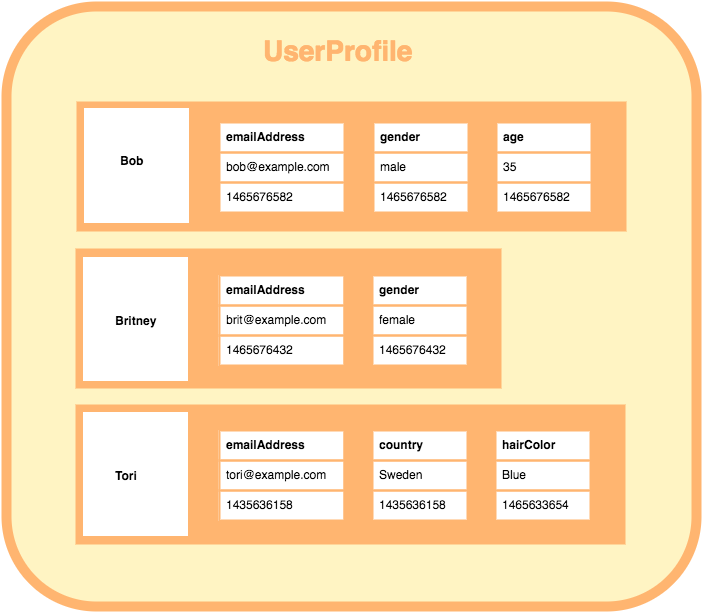
\includegraphics[width=0.75\columnwidth]{img/wide_column_store.png}
    \caption{Example entity relation model \autocite{wideColumnGraphic}}
    \label{fig:cassandra:wide_column}
\end{figure}

Figure~\ref{fig:cassandra:wide_column} shows in a graphical representation the structure of a wide column store. The name is the primary key and different people have different columns. The columns with no data are not stored as null but rather not even stored as a whole.

\section{Use-Cases Cassandra}
Cassandra comes with strong benefits over other database systems. These benefits and extra features make it miss some features which one might expect as standard in database systems.
It should be carefully considered whether to use Cassandra or not since it is not the jack of all trades.
One benefit of Cassandra is fast writes which means it can handle a high throughput but the latency might not be too short. These writes include the operations of {INSERT}, {UPDATE} and {DELETE}.
The way Cassandra handles those operations make them equal to a "regular" write operation. This will be explained in section \ref{sec:cassandra:cql}. Another key benefit is high availability. Due to its architecture and depending on the settings, a Cassandra setup can be highly available. Since one of the base assumptions of a distributed system is the expensiveness of inter-node communication, it has an linear horizontal scalability.
The communication between nodes does not increase with the size of node. Due to its distributed nature, the architecture does not rely on a master-slave setting and comes masterless.
Furthermore it can be configured to work with several clusters, globally distributed, which makes for example multicloud Cassandra setups possible.
This means that any client can read from and write to any node. As described previously Cassandra is a wide column store database which results in having a flexible schema where rows can have missing columns that are not stored on disk.
Cassandra has its own query language which is similar \gls{sql} and called \gls{cql}. This makes it easier to use Cassandra if knowledge from \gls{sql} is available.

If any of these points apply to a project or Use-Case, Cassandra is probably a good fit.
But to be sure it is even more important to rule out the cases where Cassandra is not a good fit.
The following paragraph will describe limits of Cassandra. If the use-case needs any of those features, Cassandra will most likely not suffice to fulfill requirements.
First, a single system instance with Cassandra should be avoided. Most of the features and benefits come with multiple node setups. Use-Cases which would need a dozen nodes seem to find a great fit with the distributed storage system.

Equally important is the way data has to be stored and accessed. Due to its architecture, data has to be modeled different in Cassandra. \acrshort{acid} transactions are not possible and tables are fine-tuned for pre defined queries. Those queries should be known early on and not change during use. It is not easily possible to change or extent those queries. Furthermore there are no relations between tables. It is possible to link, connect and reuse IDs but this has to be handled on client side, there are no operations on those IDs available. Additionally column aggregation operations such as \texttt{GROUP BY} are also not possible, since such operations would be very inefficient in a distributed wide column storage.

Having a lot of updates and deletes interspersed with reads slow the system down due to the way of handling requests - just appending data, not changing records and merging them while reading. This has affects on data validation as well. It is not possible to check on write for data uniqueness, constraints or auto increments. \autocite{cassandra_oreilly}

To sum it up there are general Use-Case conditions where Cassandra is a great fit.
In order to make an educated decision the following key-points should fit with the Use-Case and environment:

\begin{itemize}
    \item Large Deployments
    \item High write throughput
    \begin{itemize}
      \item{"High performance at high write volumes with many concurrent client threads"} \autocite{cassandra_oreilly}
    \end{itemize}
    \item Geographical distribution of data and database clients
    \item Different columns per row
\end{itemize}


\section{Data Modeling in Cassandra}  % How to model data (or rather tables)

Compared to other database systems like traditional relational database systems, data modeling is different in Cassandra. Here is a little example to understand the different way of thinking when modeling data for Cassandras wide column data store.

Figure~\ref{fig:cassandra:model_data0} shows an example entity relationship diagram of data in the context of a hotel environment. The hotel has the attributes \textit{address}, \textit{phone}, \textit{name} and an \textit{id} as unique primary key. Each hotel has certain amounts of rooms which store information them-self and are connected to other entities.

\begin{figure}[H]
    \centering
    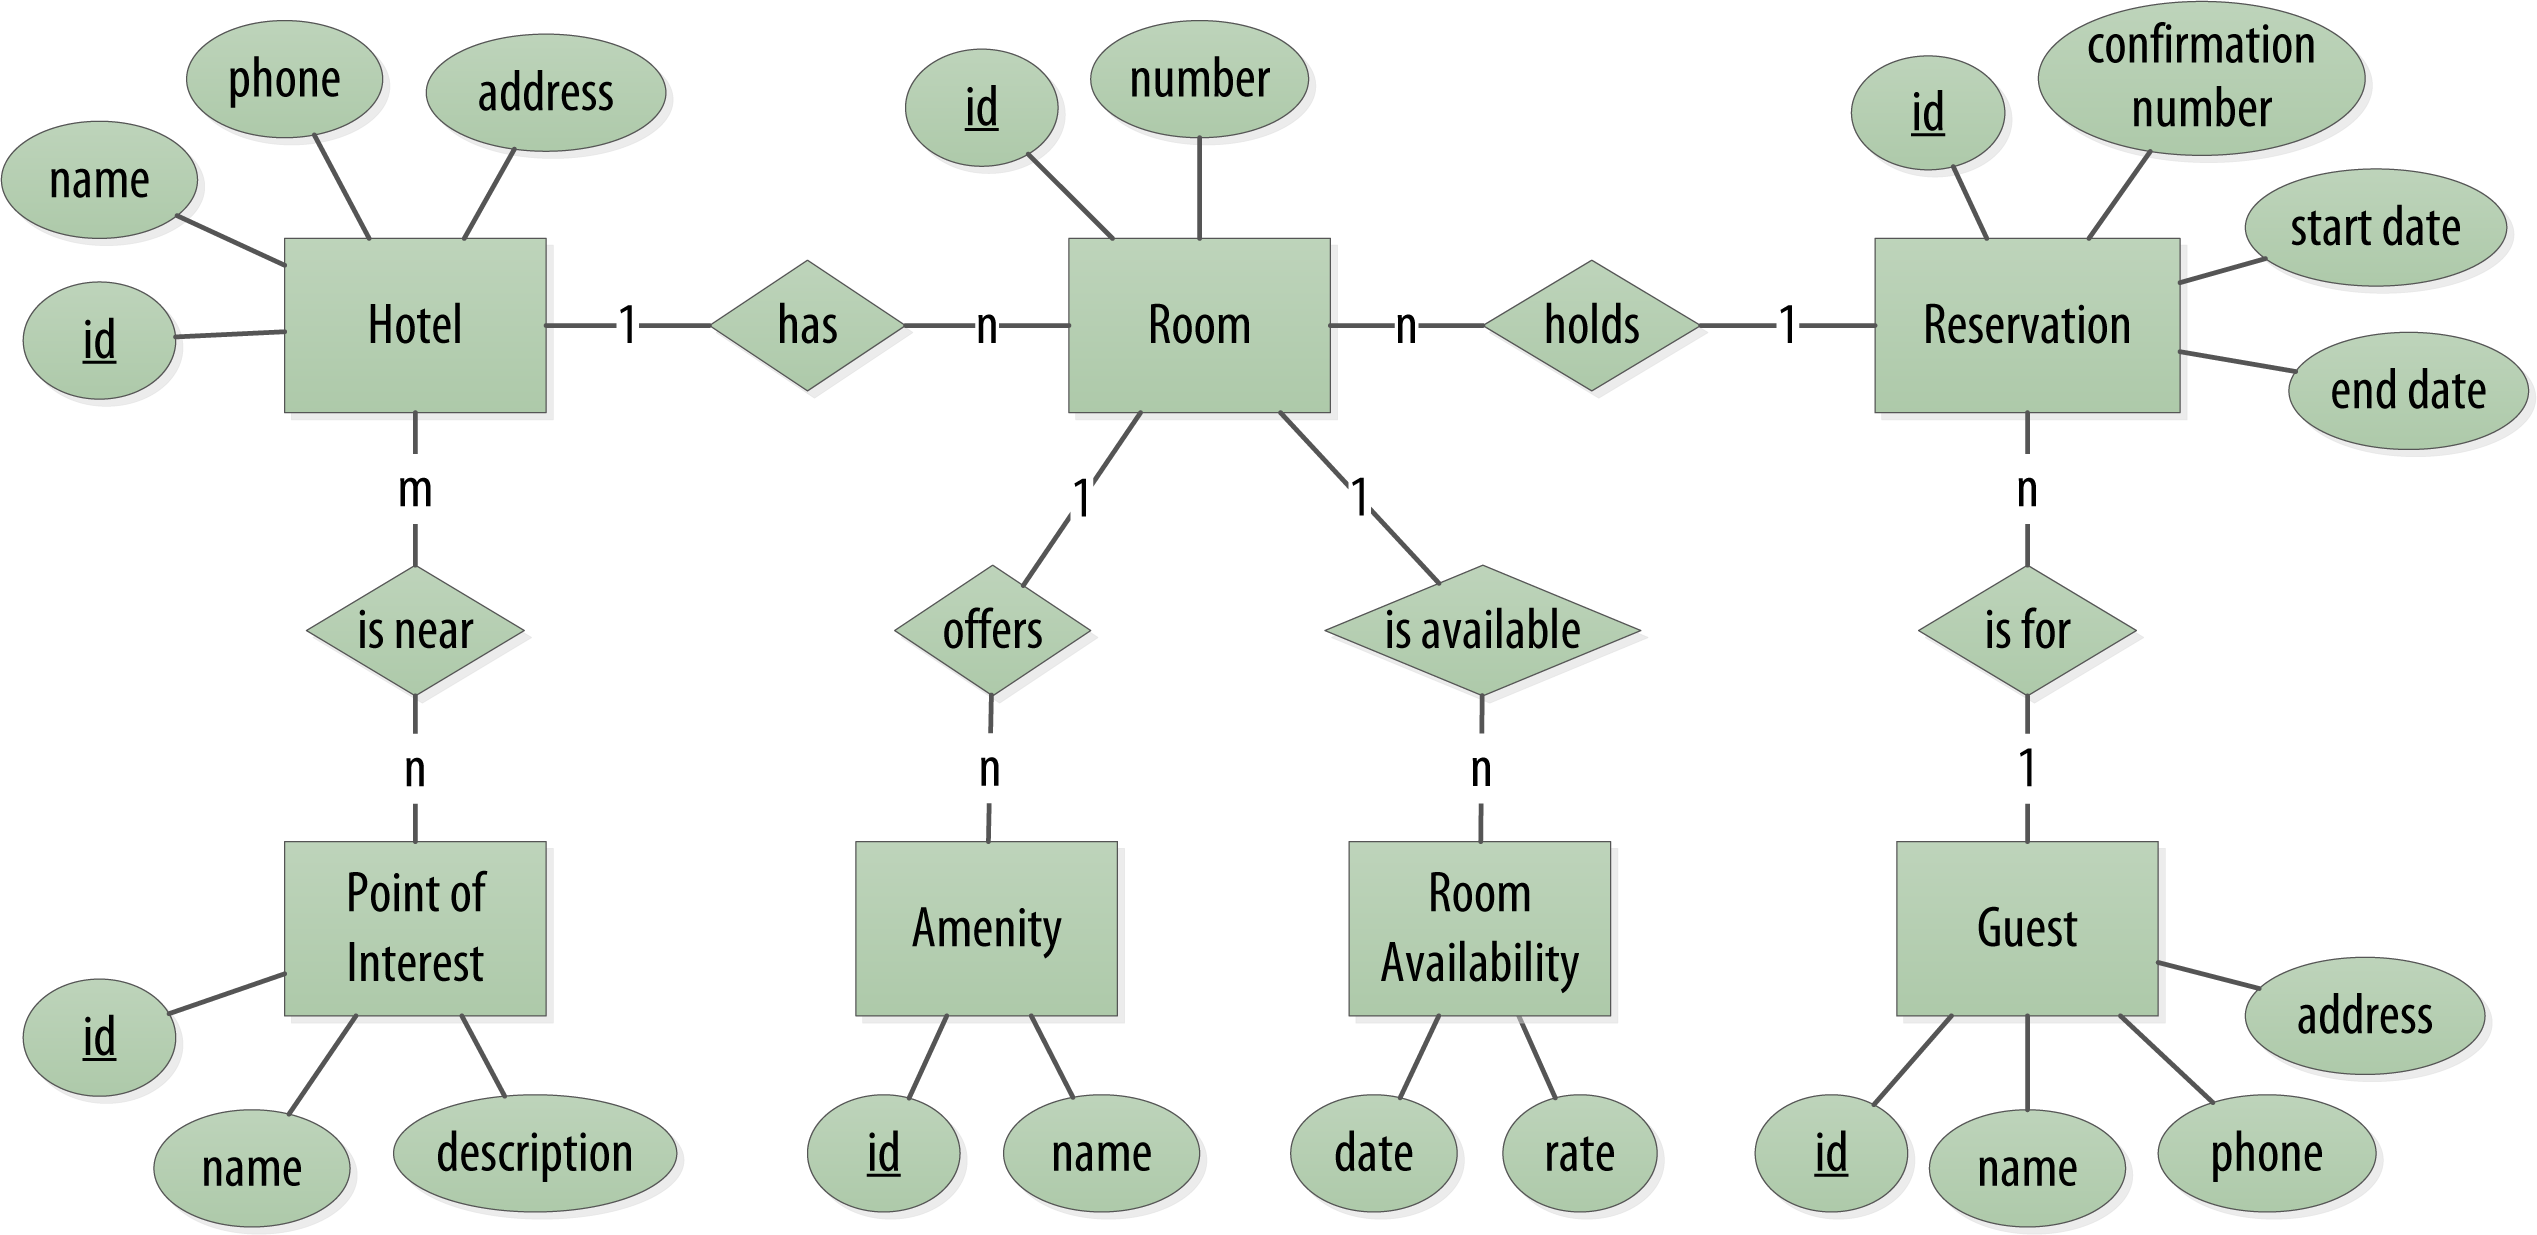
\includegraphics[width=0.75\columnwidth]{img/model_example_entity_relation_step0.png}
    \caption{Example entity relation model \autocite{cassandra_oreilly}}
    \label{fig:cassandra:model_data0}
\end{figure}

In figure~\ref{fig:cassandra:model_data1} an example database model for an relational database of the ERP from figure~\ref{fig:cassandra:model_data0}.
The connections and primary keys previously noted connect now the table to enable complex join queries over multiple tables later on.

\begin{figure}[H]
    \centering
    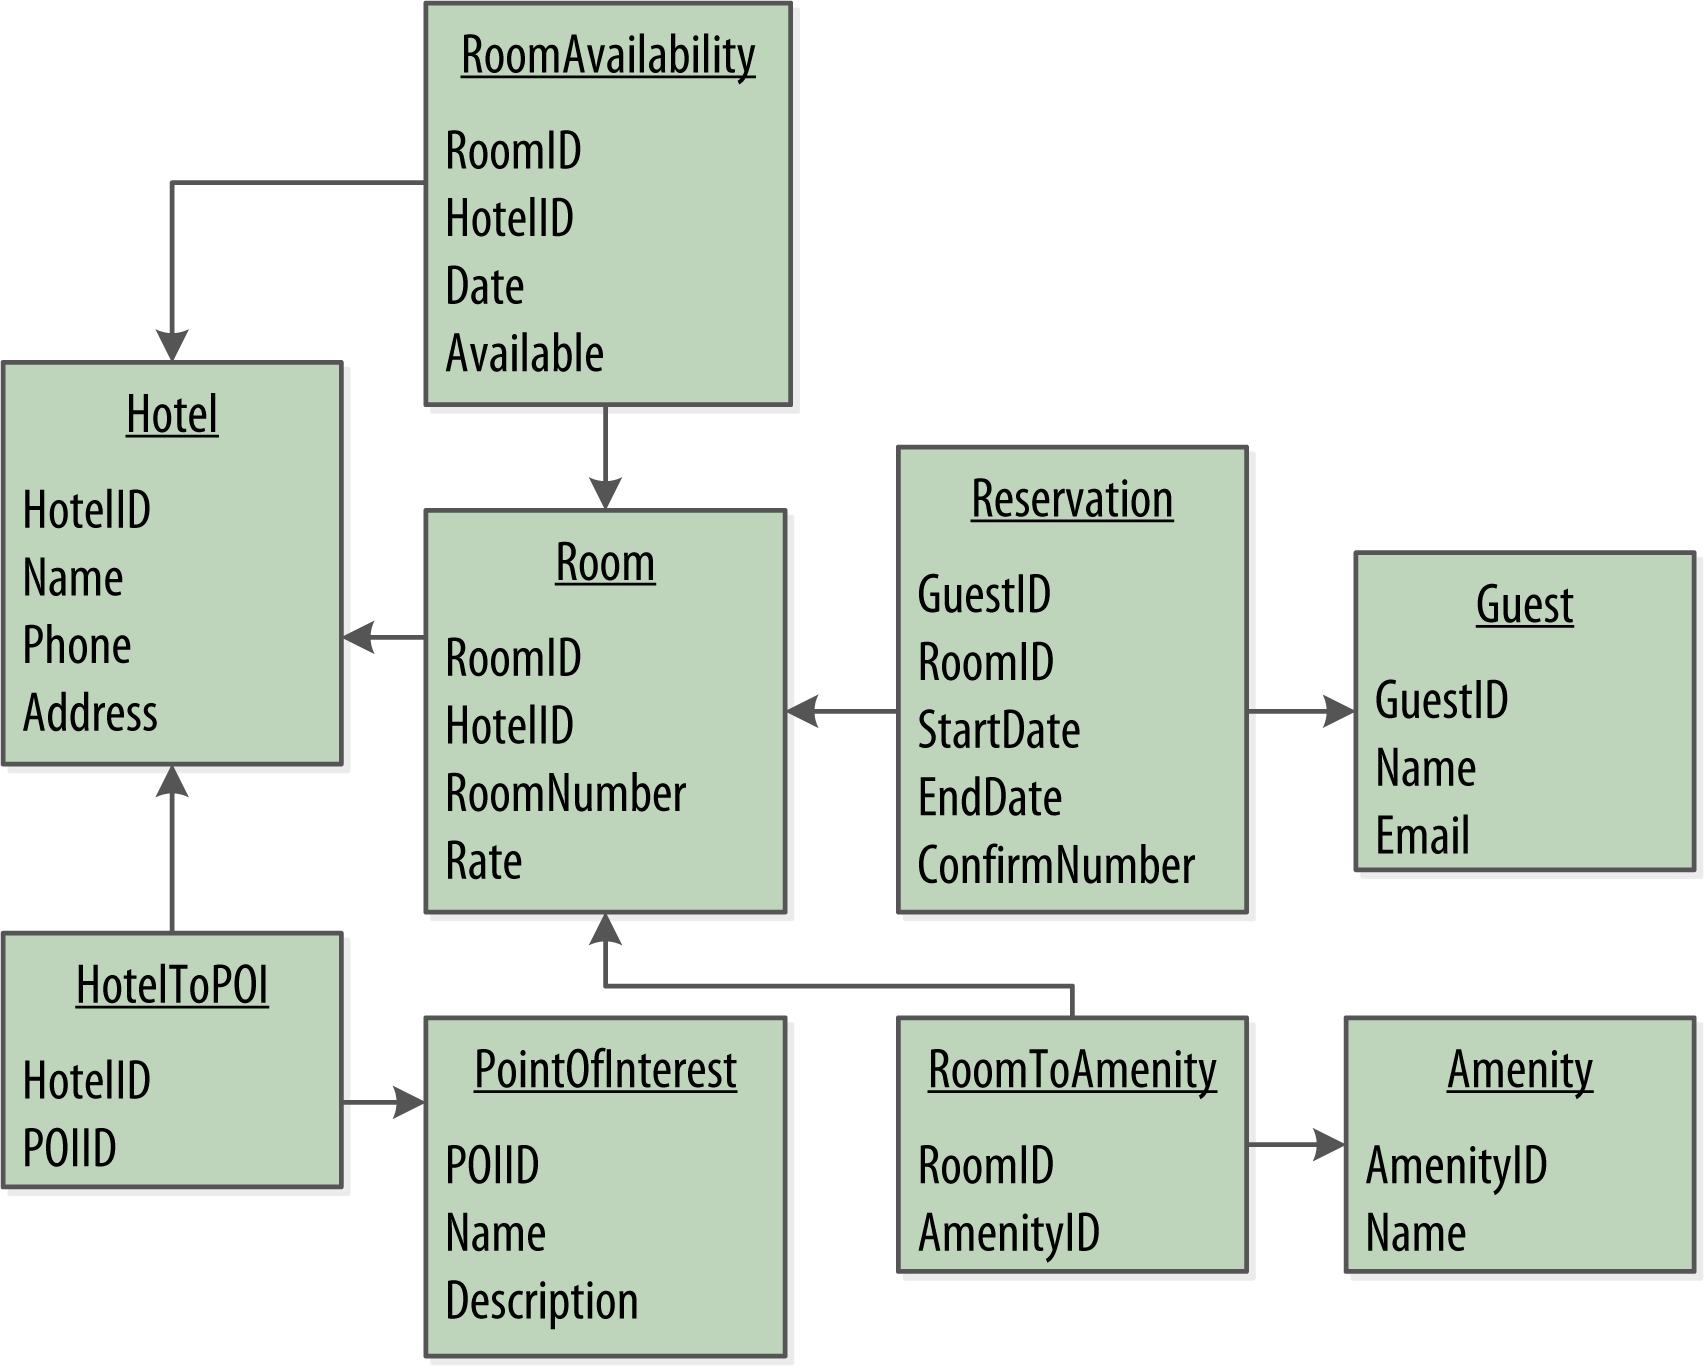
\includegraphics[width=0.75\columnwidth]{img/model_example_rdbms_step1.png}
    \caption{Example RDMBS normalization transition \autocite{cassandra_oreilly}}
    \label{fig:cassandra:model_data1}
\end{figure}

The fundamental difference between those two modeling types is the starting point. In the example above it was all about what data has to be stored and how that data is connected to each other.
In data modeling for Cassandra the queries are the starting points. This means for the architect that they first have to think about queries the database system has to answer.

\begin{figure}[H]
    \centering
    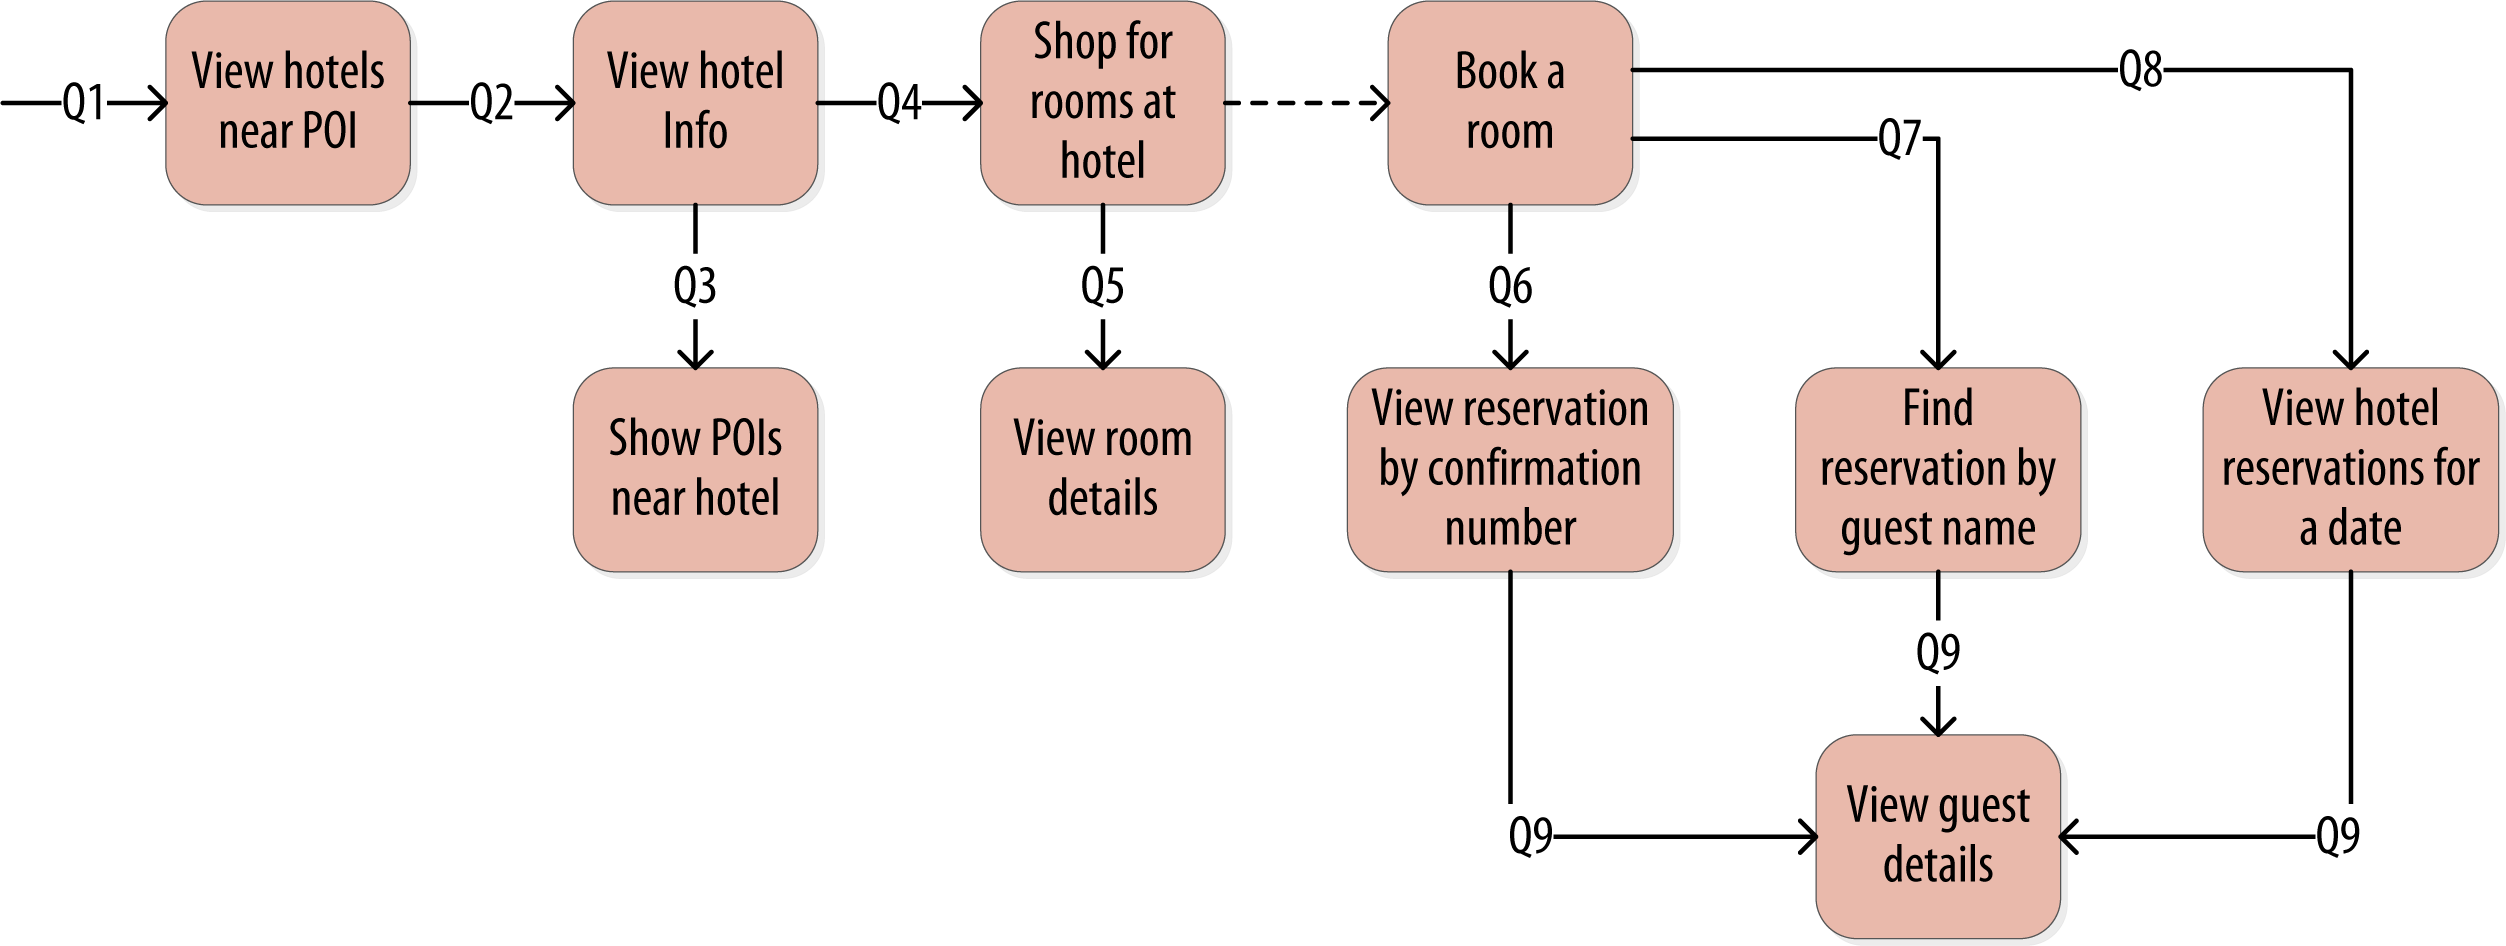
\includegraphics[width=0.75\columnwidth]{img/model_example_queries_step2.png}
    \caption{Planned queries against database system \autocite{cassandra_oreilly}}
    \label{fig:cassandra:model_data2}
\end{figure}

Figure~\ref{fig:cassandra:model_data2} show this circumstance; queries the system later has to answer to. This diagram describes a classical use-case for the hotel environment in which the database would come to work. A user searches for hotels, checks information about it and reserves it.

\begin{figure}[H]
    \centering
    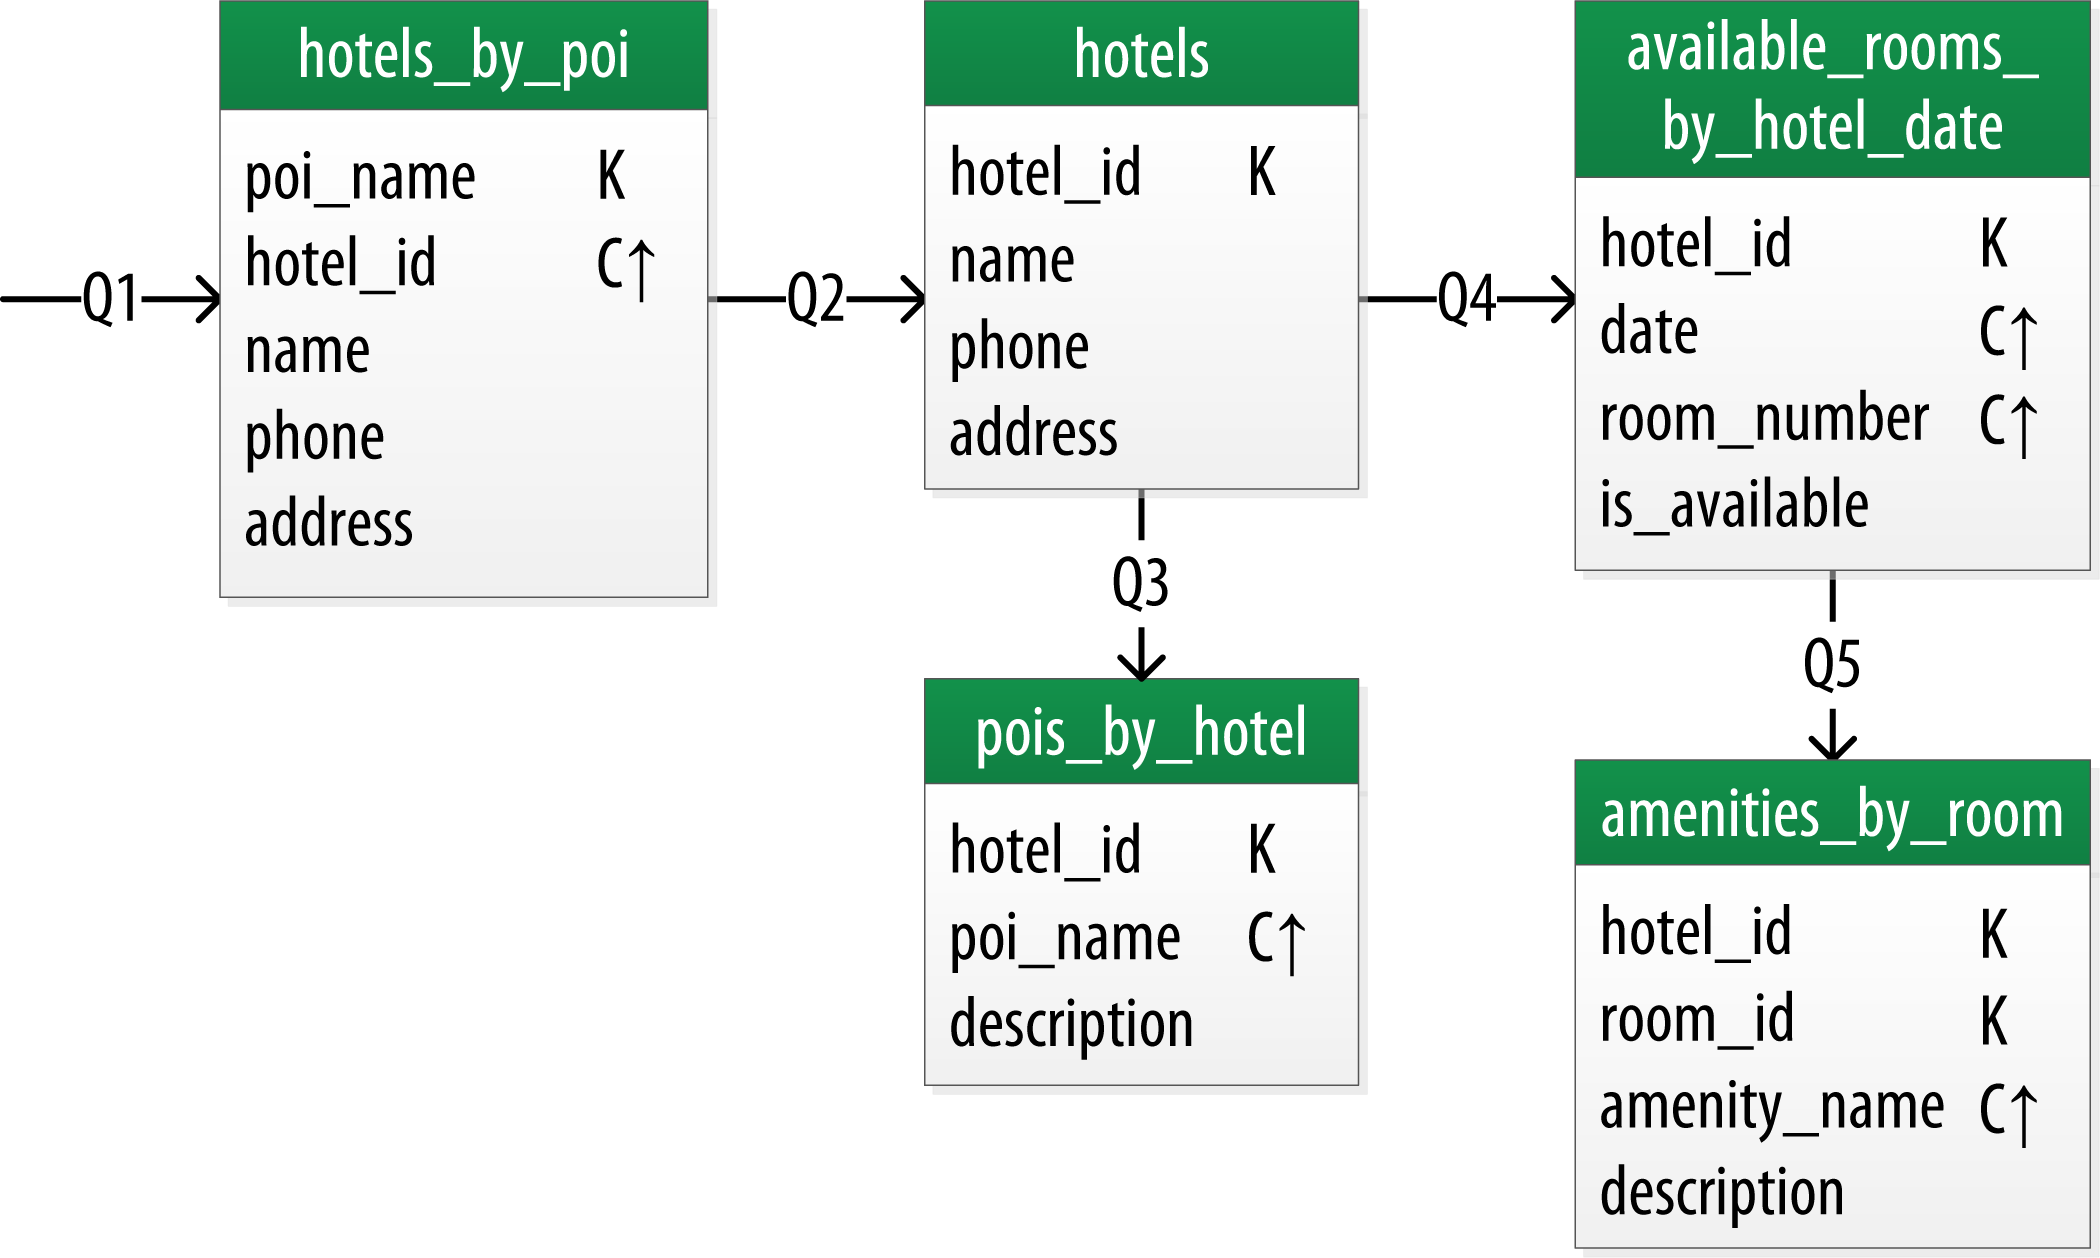
\includegraphics[width=0.75\columnwidth]{img/model_example_chebotko_step3.png}
    \caption{Model and denormalize tables to fit queries \autocite{cassandra_oreilly}}
    \label{fig:cassandra:model_data3}
\end{figure}

Transitioning from the collection of queries in figure~\ref{fig:cassandra:model_data2} to accessible tables, can be seen in figure~\ref{fig:cassandra:model_data3}. It can be seen that data is stored redundantly, available on multiple tables. This does not bother the modeling since queries later on will not use any sort of join operation and be limited onto one table request - which is precisely why data is stored in multiple tables. Each table fulfills one of the queries previously thought of. Furthermore since there is no referential integrity it is possible to store \textit{ids} in tables but the database system does not provide any functionality to make use of and / or connect those \textit{ids}.

In order to properly graph and document this type of modeling, a uniform and new way was proposed to write down data modeling for Cassandra and other similar systems with same needs. \autocite{chebotko2015data}
These diagrams are called Chebotko diagrams and include the way queries are planned. This can be seen in figure~\ref{fig:cassandra:model_data2}.
Out of this table, the diagram can be concluded. Creating to each query an unique table with all necessary information. The arrows with the queries numbers (Q1, Q2 ..) will be kept to keep the context and relation to the previous diagram (\ref{fig:cassandra:model_data3}).
This can be seen in a descriptive example section around figure~\ref{fig:cassandra:chebotko}

\begin{figure}[H]
    \centering
    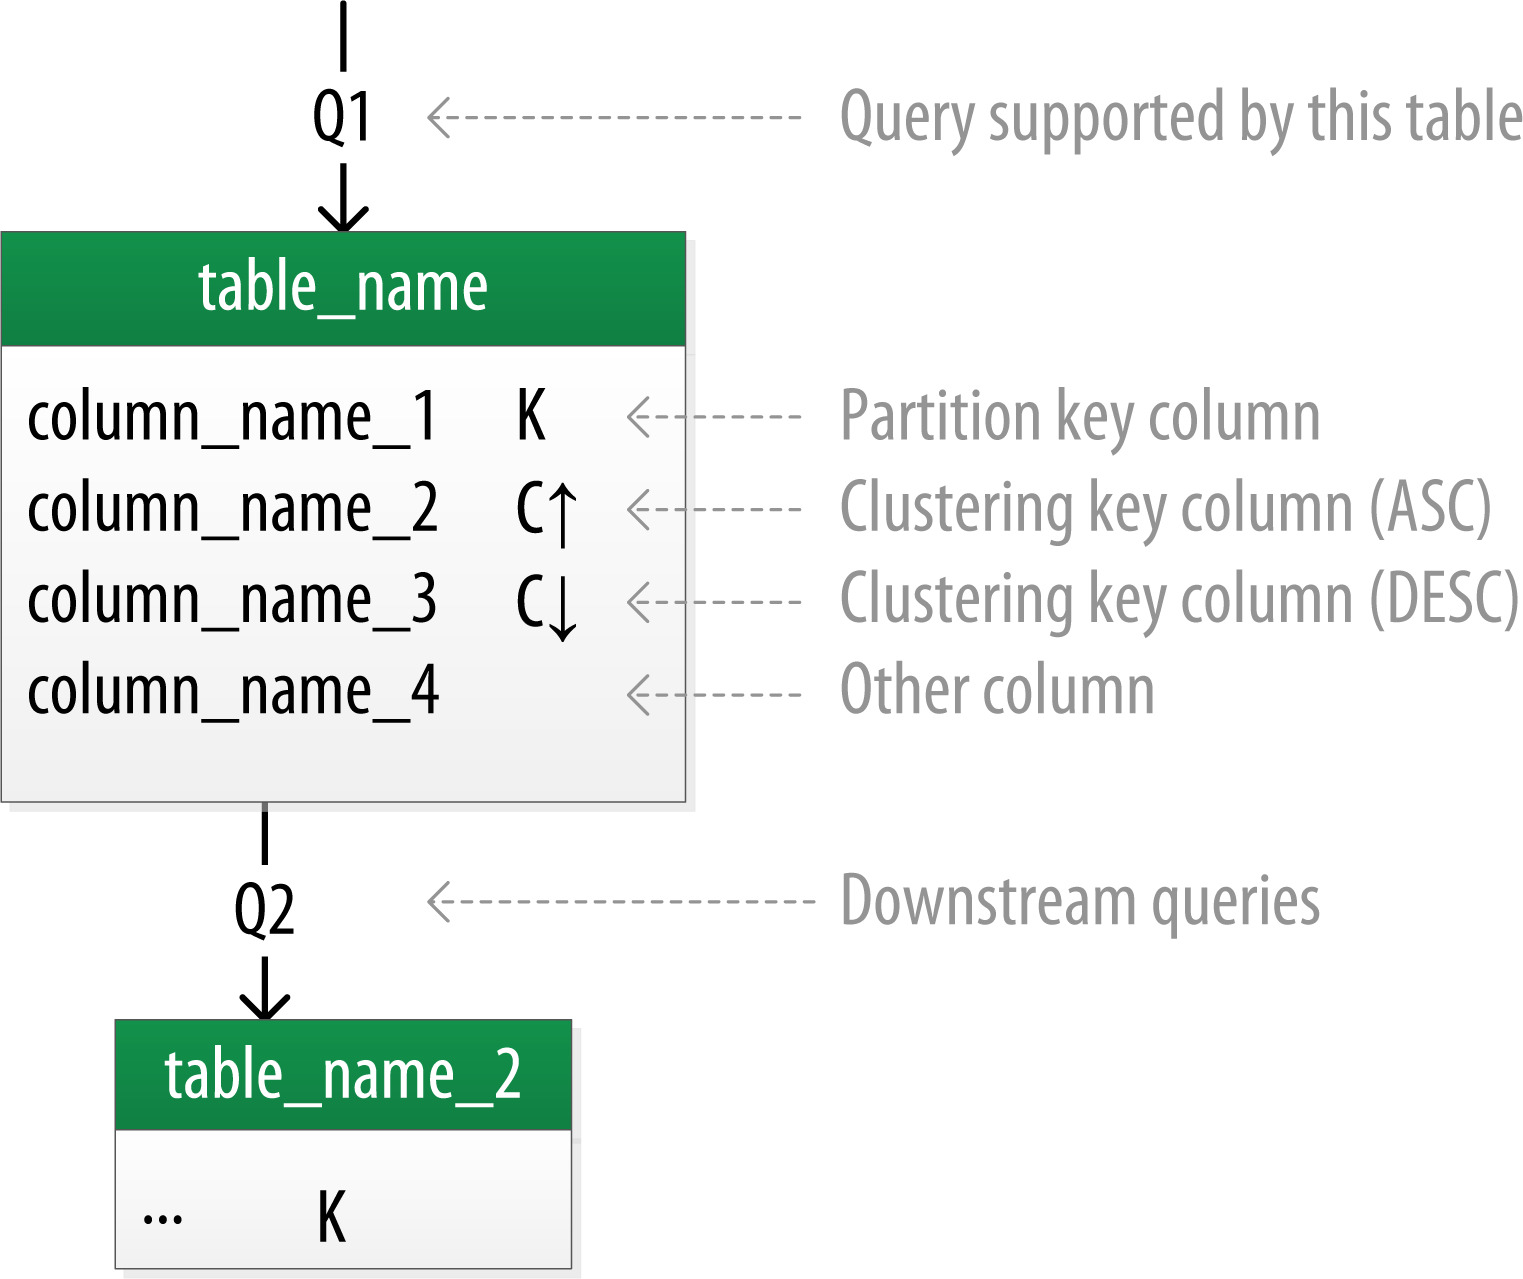
\includegraphics[width=0.75\columnwidth]{img/model_example_primary_key.jpeg}
    \caption{Model and denormalize tables to fit queries \autocite{cassandra_oreilly}}
    \label{fig:cassandra:chebotko}
\end{figure}

\section{Using the Cassandra Query Language} \label{sec:cassandra:cql} % How to use CQL
This section will give a short overview of how to interact with a Cassandra database using \gls{cql}, which is mainly inspired by \gls{sql} \autocite{cqlAlexMeng, newInCQL3, cassandra3cqldocCreateKeystore}.

\subsection {Creating a keyspace}
This similarity becomes clear by looking at how the creation of a keyspace is performed:
\begin{verbatim}
/* Create a new keyspace in CQL */
CREATE KEYSPACE data WITH replication =
    {'class': 'SimpleStrategy', 'replication_factor': 3};

/* Create a new database in SQL */
CREATE DATABASE data;
\end{verbatim}

Hereby the only difference is that instead of creating a database, a keyspace is created and it is possible to specify which replication parameters should be used. What these parameter mean and how they should be used is explained later in section~\ref{sec:CassandraClusterArchitecture} \autocite{cqlAlexMeng}.

\subsection{Creating a table}
After creating a keyspace a table has to be created in order to hold the data. As a database is always part of a keyspace it is either necessary to specify the keyspace in every query or to simple scope every subsequent query into a given keyspace by using the USE query \autocite{cassandra3cqldocUse}:
\begin{verbatim}
USE data;
\end{verbatim}

Using this keyspace a table can be created using the same syntax as in \gls{sql} \autocite{cqlAlexMeng, newInCQL3, cassandra3cqldocCreateTable}:
\begin{verbatim}
CREATE TABLE groups (
   group_name varchar,
   group_location varchar,
   added_date date,
   username varchar,
   PRIMARY KEY (...)
);
\end{verbatim}

Hereby the only difference is how the primary key can be specified:

\begin{figure}[ht]
    \centering
\begin{verbatim}
      partition key       clustering key  clustering key
       |       |                |            |
((groupname, group_location), added_date, username)
\end{verbatim}
    \caption{Parts of a primary key specification in \gls{cql} \autocite{cqlPrimaryKeyDefinition}}
    \label{fig:cassandra:primaryKeyDefinition}
\end{figure}

The first part of the definition will always be the partition key. If it is a compound of several columns they need to be surrounded by parentheses and separated by comma in order to state that they as a whole form the partition key. If necessary the partition key can be followed by several clustering keys. Keep in mind that the data will be ordered first by the first clustering key, after that by the second and so on. This means that an \texttt{ORDER BY} has to first be called on the first clustering key and a second ordering can be done on the subsequent one. It will not be possible to only order by the second or other subsequent clustering keys when not ordering by the first. Any other non-primary key column cannot be used for ordering \autocite{cqlPrimaryKeyDefinition, cassandra3cqldocCreateTable}.

\subsection{Interacting with data}
In order to manipulate Cassandra only provides three possible methods \autocite{lakshman2010cassandra}:
\begin{itemize}
    \item insert(table, key, rowMutation)
    \item get(table, key, columnName)
    \item delete(table, key, columnName)
\end{itemize}
All having in common that the entire primary key has to be specified in order to interact with the data. The only exception hereby is the getting of data where only the partition key has to be specified.

Important to note is that there is no interaction to update a data entry. The reason for that is that as Cassandra is optimized for high write throughput is is very costly to read any data before writing. This means that the update and insert known from \gls{sql} will perform the same action on the data \autocite{cqlAlexMeng, newInCQL3}:
\begin{verbatim}
/* Inserting Data */
INSERT INTO Person (lastname, name, email)
  VALUES ('Doe', 'Jane', 'jane@example.com');

/* Updating Data */
UPDATE Person SET email = 'jane@example.com'
  WHERE lastname='Doe' AND name = 'Jane';
\end{verbatim}

As getting and deleting data is also similar to \gls{sql} there is no need to go into it any further in this section \autocite{cqlAlexMeng, cassandra3cqldocSelect}:
\begin{verbatim}
/* Selecting Data */
SELECT * FROM Person
  WHERE lastname='Doe' AND name = 'Jane';
/* Deleting Data */
DELETE FROM Person
  WHERE lastname='Doe' AND name = 'Jane';
\end{verbatim}

\section{Local reads and writes}
In order to perform the requested changed to the data they have to be written into the database. This section will take a look into how the changes will be written on a single node not taken into account the cluster.

\begin{figure}[ht]
    \centering
    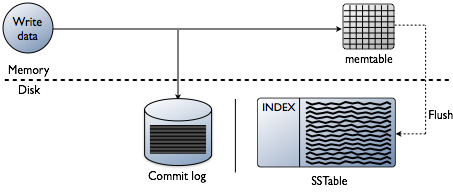
\includegraphics[width=0.75\textwidth]{img/cassandra_local_write.png}
    \caption{Writing data to Cassandra node \autocite{datastaxWriteData}}
    \label{fig:cassandra:writeData}
\end{figure}
In figure~\ref{fig:cassandra:writeData} it can be seen that the write process to Cassandra involves three steps:
\begin{enumerate}
\item \textbf{Write to journal} Hereby the query is simple append to the journal on the disk, making it persistent even if the node goes down. As this action is a simple append it is very fast and leaves the data in a temporal order in the journal.
\item \textbf{Write to memtable} After writing to the journal the change is performed in the memtable putting the data into a Sorted String Table (SSTable). This form is the same form in which the data will be written on disk. Here it is important that only the required data is written if there are any columns not specified it will not be written to the memtable. In contrast to writing \texttt{NULL} to a column which will delete it by setting a tombstone on it (See Appendix \ref{appendix:cassandra:queryExample}).
\item \textbf{Flush to disk when memtable is too big} This allows to simply flush the data and some metadata to the disk when it gets to big for the memory to hold it. Hereby a new data file is created, not touching any of the previously written files, making this action also quite fast as no lookups have to be performed.
\item \textbf{Compacting written datafiles} As writing to disk is only an append and will create a new datafile for every flush, the whole database will be scattered over multiple files with redundant data if entries were written after flushing them to disk. In order to merge these files it is possible to compact the files into one resulting in faster reads later \autocite{cassandraCompactTool}.
\end{enumerate}

After writing the data it also can be read again as shown by figure~\ref{fig:cassandra:readData}:

\begin{figure}[ht]
    \centering
    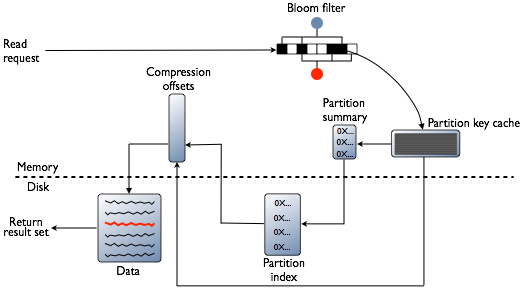
\includegraphics[width=0.75\textwidth]{img/cassandra_local_read.png}
    \caption{Reading data from Cassandra node \autocite{datastaxReadData}}
    \label{fig:cassandra:readData}
\end{figure}
\begin{enumerate}
    \item \textbf{Check caches} First the last query cache will be checked. Returning the data right away if it was requested in the near past.
    \item \textbf{Check memtable} If not found in the caches the memtable will be checked whether it has the most recent activities on the requested data.
    \item \textbf{Find SSTable and location} If no entry was found in the memtable the data on disk will be checked by firstly determining in which memtable dump the dataset will be and then retrieving it from there. For a detailed overview of this take a look at figure \ref{fig:cassandra:readData}
    \item \textbf{Merge with memtable} If it was necessary to retrieve the data from disk the data will be written to the memtable to allow later queries on the same data to succeed earlier.
\end{enumerate}

\section{Cluster Architecture}\label{sec:CassandraClusterArchitecture}  % How the cluster works
Which node has a certain piece of data is not determined by a master server. Any node has the ability to determine where a particular piece of data is or must be stored just by hashing the partition key of a row. The result of that calculation is called a token. All nodes are placed somewhere on a \textit{token ring} (see figure~\ref{fig:cassandra:tokenring}) and store the data of the tokens they are assigned to.\autocite[2]{lakshman2010cassandra} \autocite[209,210]{DeCandia2007Dynamo}

\newcommand{\Ray}{3cm}
\begin{figure}[ht]
  \centering
  \begin{tikzpicture}
    % Nodes on the circles
    \node[circle,minimum width=2cm,minimum height=1cm,draw,name path=n1] (Node A) at (90:\Ray) {A};
    \node[circle,minimum width=2cm,minimum height=1cm,draw,name path=n2] (Node B) at (0:\Ray) {B};
    \node[circle,minimum width=2cm,minimum height=1cm,draw,name path=n3] (Node C) at (270:\Ray) {C};
    \node[circle,minimum width=2cm,minimum height=1cm,draw,name path=n4] (Node C) at (180:\Ray) {D};

    % Circle the nodes are placed on
    \path[name path=c] circle (\Ray);
    \path[name intersections={of=n1 and c,name=i1},
          name intersections={of=n2 and c,name=i2},
          name intersections={of=n3 and c,name=i3},
          name intersections={of=n4 and c,name=i4}
         ];

    % Arrows between the nodes
    \begin{scope}
      \pgfsetarrowsend{Stealth[scale=1.5]}

      \pgfpathmoveto{\pgfpointanchor{i1-2}{center}}
      \pgfpatharcto{\Ray}{\Ray}{0}{0}{0}{\pgfpointanchor{i2-1}{center}}
      \pgfusepath{draw}

      \pgfpathmoveto{\pgfpointanchor{i2-2}{center}}
      \pgfpatharcto{\Ray}{\Ray}{0}{0}{0}{\pgfpointanchor{i3-1}{center}}
      \pgfusepath{draw}

      \pgfpathmoveto{\pgfpointanchor{i3-2}{center}}
      \pgfpatharcto{\Ray}{\Ray}{0}{0}{0}{\pgfpointanchor{i4-2}{center}}
      \pgfusepath{draw}

      \pgfpathmoveto{\pgfpointanchor{i4-1}{center}}
      \pgfpatharcto{\Ray}{\Ray}{0}{0}{0}{\pgfpointanchor{i1-1}{center}}
      \pgfusepath{draw}
    \end{scope}

    % Labels on arrows
    \node[fill=white] at (45:\Ray) {0 to 63};
    \node[fill=white] at (135:\Ray) {64 to 127};
    \node[fill=white] at (225:\Ray) {128 to 191};
    \node[fill=white] at (315:\Ray) {192 to 255};
  \end{tikzpicture}
  \caption{Token Ring}
  \label{fig:cassandra:tokenring}
\end{figure}

The tokens from the node's location to the next node belong to it. That means if the hashing of a partition key results in a token between 0 and 63 the data will be written to or read from node A. Keep in mind: This doesn't however mean that this node is \textit{in control} of that data - when replication is configured all replicas are equal. The node with that token is just the starting point to determine the first of the replicas.

\paragraph{Replication} To ensure that all data continues to be available even if some nodes go down Cassandra replicates the data in the cluster. Replication can be defined for each keyspace when it is created. There is a simple strategy and a network topology aware strategy. \autocite{datastax_replication} \\
The \texttt{SimpleStrategy} places the $n$ replicas of a piece of data on the next $n-1$ nodes\footnote{The first node that holds the data also counts as a replica.} located clockwise on the ring after the node with the token. \autocite[3]{lakshman2010cassandra} \\
The \texttt{NetworkTopologyStrategy} strategy tries to be smart about the physical placement of replicas. It needs to be taught about in which datacenter and rack the nodes are located. To avoid losing data when an entire rack or datacenter fails this strategy prefers to spread it out.
It is recommended to use this strategy in production, unless all nodes are in a single rack, where both strategies are equivalent.

\paragraph{Rebalancing}

When a new node is added or a node is removed it is likely that the distribution of nodes on the ring becomes imbalanced. When the ring is imbalanced nodes are responsible for different amounts of data and experience different amounts of load. Since nodes are recommended to be of the same performance level\footnote{Or be balanced by dividing them up into virtual nodes according to performance} this is not optimal. Some nodes are overloaded and others underutilized.
To balance the ring the nodes are moved to equidistant positions on the ring. When this happens data is bound to be assigned to a new owner node - that data will be moved. \autocite{datastax_balancing}
The hash function used to transform partition key into is a so called \textit{consistent hash function}. The difference from a regular (cryptographically secure) hash function is that the output wraps around and thus can be represented as a ring. It also has the property that it minimizes the amount of shifting data that is necessary when a node is added or removed. \autocite{karger1997consistent}

Figure~\ref{fig:cassandra:rebalancing} visualizes an imbalanced ring and how the green nodes can be repositioned.


\begin{figure}[ht]
  \centering
  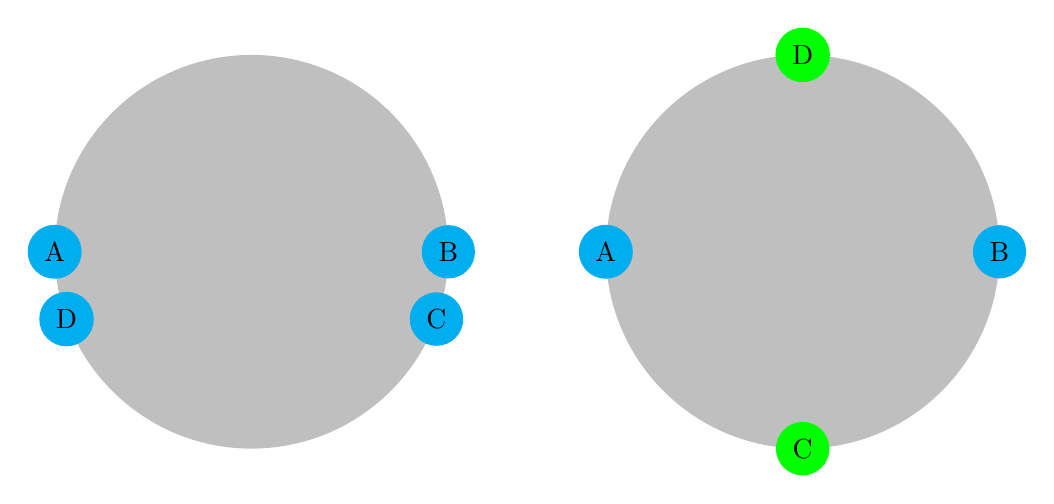
\begin{tikzpicture}
    % Circle
    \fill[fill=black!25] (2.5, 0) arc (0:360:2.5);
    \node[circle,fill=cyan] at (180:2.5) {A};
    \node[circle,fill=cyan] at (0:2.5) {B};
    \node[circle,fill=cyan] at (-20:2.5) {C};
    \node[circle,fill=cyan] at (200:2.5) {D};

    % Legend
    \begin{scope}[shift={(7,0)}]
      \fill[fill=black!25] (2.5, 0) arc (0:360:2.5);
      \node[circle,fill=cyan] at (180:2.5) {A};
      \node[circle,fill=cyan] at (0:2.5) {B};
      \node[circle,fill=green] at (270:2.5) {C};
      \node[circle,fill=green] at (90:2.5) {D};
    \end{scope}
  \end{tikzpicture}
  \caption{Rebalancing}
  \label{fig:cassandra:rebalancing}
\end{figure}

Nodes A and B can stay at their location, C and D are repositioned. C is moved further along the ring in a clockwise direction. It gives much of the data it was previously responsible to B and takes all of D's data. D is moved past A and takes approximately half of its data.

\paragraph{Virtual Nodes}

By default each node is placed on the ring just once, when using virtual nodes they each can be placed on the node multiple times. This brings four advantages: \autocite{datastax_vnodes, yelp_balancing}

\begin{itemize}
  \item Nodes can occupy a specified proportion of the ring
  \item Tokens are automatically calculated and assigned to nodes $rightarrow$ No manual rebalancing
  \item Data hotspots on the ring are handled my multiple nodes
  \item Rebuilding of replacements is faster
\end{itemize}

1. When nodes have different processing capabilities and disk space that performance difference should be taken into account so that all nodes receive load which is proportional to their performance. With virtual nodes enabled a node can be assigned any number of tokens. Not the absolute number of tokens of an individual node is relevant it only has an effect on how much of the ring it occupies on relation to the others.  \\
2. Without using virtual nodes the tokens for each node have to be calculated manually and assigned to each node. Cassandra also automatically rebalances the ring whenever a new node joins or a node leaves. \\
3. When data partitioning was done poorly or the data happens to cluster around a particular token range the node responsible for that data receives disproportionately much load. Virtual nodes remedy that because they not only make the individual partitions smaller but they also make any single note responsible for multiple areas on the ring. \\
4. When a node goes down and a replacement is brought up. This replacement needs the data of the node it replaced. If the replication factor is three it needs data from three different partitions. Without virtual nodes this can come from up to $3\cdot(3-1)=6$ different replicas. When using virtual nodes the partitions the same amount of data is spread across more nodes and thus the replication can transfer data from more nodes at once. If each node is split into $k$ virtual nodes it can replicate from $k$ times more replicas.

See figure~\ref{fig:cassandra:vnodes} for a visualization.

\begin{figure}[ht]
  \centering
  \begin{tikzpicture}
    % Circle
    \draw[line width=1.5mm] (\Ray, 0) arc (0:360:\Ray);

    % Nodes on the circle
    \foreach \x [count=\p] in {0,...,2} {
      \node[circle,draw,minimum size=1cm,fill=orange] at (90-\x*120-0*30:\Ray)
        {\pgfmathparse{1+4*\x}\pgfmathprintnumber{\pgfmathresult}};
      \node[circle,draw,minimum size=1cm,fill=cyan] at (90-\x*120-1*30:\Ray)
        {\pgfmathparse{2+4*\x}\pgfmathprintnumber{\pgfmathresult}};
      \node[circle,draw,minimum size=1cm,fill=yellow] at (90-\x*120-2*30:\Ray)
        {\pgfmathparse{3+4*\x}\pgfmathprintnumber{\pgfmathresult}};
      \node[circle,draw,minimum size=1cm,fill=black!25] at (90-\x*120-3*30:\Ray)
        {\pgfmathparse{4+4*\x}\pgfmathprintnumber{\pgfmathresult}};
    };

    \node[circle,draw,minimum size=1cm,fill=orange,label=right:{Node A}] at (2*\Ray, 1.875) {};
    \node[circle,draw,minimum size=1cm,fill=cyan,label=right:{Node B}] at (2*\Ray, 0.625) {};
    \node[circle,draw,minimum size=1cm,fill=yellow,label=right:{Node C}] at (2*\Ray, -0.625) {};
    \node[circle,draw,minimum size=1cm,fill=black!25,label=right:{Node D}] at (2*\Ray, -1.875) {};
  \end{tikzpicture}
  \caption{Virtual Nodes}
  \label{fig:cassandra:vnodes}
\end{figure}

\subsection{Distributed writes and reads (CAP Theorem)} \label{subsec:cassandra:cap}

Cassandra has a masterless architecture; no single node controls any particular piece of data \autocite[5]{lakshman2010cassandra}\footnote{Unless explicitly configured to do so}. A consequence is that a client can run queries against any node of the cluster. In practice the client determines, either by some heuristic of proximity/latency or a round-robin algorithm, which node to use.
For one query that particular node becomes the \textit{coordinator node}; it coordinates the execution and distribution of that query.
First it hashes the partition key of the data to obtain the token and finds the node responsible for it. By using the replication strategy it can find out which replicas are responsible for that data as well. \\
When executing a read query the coordinator asks all replicas\footnote{A replica is every node responsible for that piece of data - the one determined by hashing as well as the others determined by replication strategy.} for the data. When more than \texttt{CL.read} replicas have answered the client is given an answer. When the replicas don't agree on the value of the data the client is sent the newest copy. Once all answers have come in the replicas with outdated information are sent a message on how to update their data, this is called a \textit{read repair}. \autocite{cassandra_distributed_read} \\
When executing a write query the coordinator sends the write request to all responsible replicas. If a replica is not currently available the coordinator logs the request and retries it later when the replica is back up  - this is called a \textit{hinted handoff}\autocite[6,7]{cassandraInCAPtheorem}. After more than \texttt{Cl.write} replicas have responded that they successfully completed the write the client is given a successful response. \autocite{cassandra_distributed_write}

For an explanation of the consistency levels \texttt{CL.read} and \texttt{CL.write} see section~\ref{subsec:cassandra:cap}.

In short, the process looks like this:

\begin{enumerate}
  \item Client sends query to any node
  \item That node becomes coordinator
  \item Coordinator determines tokens by hashing
  \item Coordinator sends write or read requests to all replicas determined by replication strategy
  \item For writing
    \begin{enumerate}
      \item Return success to client when more than \texttt{CL.write} nodes have acknowledged
      \item Write \textit{hinted handoff} to log for nodes that are currently unavailable
    \end{enumerate}
  \addtocounter{enumi}{-1}  % Both writing and reading should have the same number
  \item For reading
    \begin{enumerate}
      \item Return newest response when more than \texttt{CL.read} nodes have responed
      \item Send \texttt{read\_repair} to nodes with outdated data
    \end{enumerate}
\end{enumerate}

This process is also illustrated by figure~\ref{fig:cassandra:replication}.
The client queries node 4 which becomes the coordinator and then itself queries all replicas (1, 8 and 11).
When node 1 answers the default consistency level of \texttt{ONE} is satisfied and an answer is returned to the client.

\begin{figure}[ht]
  \centering
  \begin{tikzpicture}
    % Circle
    \filldraw[fill=cyan] (\Ray, 0) arc (0:360:\Ray);

    % Nodes on the circle
    \foreach \x [count=\p] in {0,...,11} {
      \def\nodeColor{orange}
      \ifnum \p=1
        \def\nodeColor{green}
      \fi
      \ifnum \p=8
        \def\nodeColor{green}
      \fi
      \ifnum \p=11
        \def\nodeColor{green}
      \fi
      \ifnum \p=4
        \def\nodeColor{yellow}
      \fi
      \node[circle,draw,scale=0.75,fill=\nodeColor] (\p) at (90-\x*30:\Ray) {\p};
    };

    % Arrows between the nodes
    \draw [->,thick] (4) to[bend right=10] (1);
    \draw [<-,thick,draw=red] (4) to[bend left=10] (1);
    \draw [->,thick, dashed, blue] (4) -- (11);
    \draw [->,thick, dashed, blue] (4) -- (8);

    % Client plus its arrows
    \node[fill=cyan,draw,minimum width=1.5cm,minimum height=1cm,rounded corners=.1cm] (Client) at (2*\Ray, 0) {Client};
    \draw [->,thick,draw=red] (4) to[bend right=10] (Client);
    \draw [<-,thick] (4) to[bend left=10] (Client);

    % Legend
    \node[circle,draw,scale=0.75,fill=yellow,label=right:{Coordinator Node}] (coordinatorLegend) at (2.5*\Ray, 0.5) {N};
    \node[circle,draw,scale=0.75,fill=green,label=right:{Replica}] (replicaLegend) at (2.5*\Ray, -0.5) {N};
  \end{tikzpicture}
  \caption{Replication}
  \label{fig:cassandra:replication}
\end{figure}

\paragraph{Tuning Consistency} By default writes and reads need to be acknowledged by only a single replica. Usually data is configured to be replicated over multiple nodes. The result is that queries to Cassandra are highly available - any particular node can fail and the request will receive a successful response. This comes at the cost that not all replicas always have the same data - a lack of consistency. \\
Because different applications have different requirements of availability and consistency Cassandra offers several parameters to adjust its alignment on that spectrum.

One of those is the consistency level. As previously mentioned in this section it determines how many nodes have to acknowledge a request until enough nodes have acknowledged completion. Consistency level for reading and writing are abbreviated as \texttt{CL.read} and \texttt{CL.write} respectively.

Cassandra offers these, but not limited to these, options. \autocite{datastax_consistency_level}

\begin{itemize}
  \item \texttt{ALL} replicas
  \item \texttt{QUORUM}: A majority of the replicas: half + 1
  \item \texttt{THREE} replicas
  \item \texttt{TWO} replicas
  \item \texttt{ONE} replicas (default)
  \item \texttt{ANY}: Only writing - At least one replica or a logged \textit{hinted handoff} if all are unavailable
\end{itemize}

In addition to these levels Cassandra also offers others that also take into account how nodes are distributed into different datacenters. \\
For each query, but usually an entire client session, the consistency level can be chosen.

The \texttt{ALL} level yields the highest consistency. Only when all replicas have responded the response is given to the client. That means either all were updated or all were asked for their current dataset. Thus there is no uncertainty about what the result is - all replicas must agree. The \texttt{ANY} consistency level is the least consistent. The data does not have to be fully written to any SSTable, memtable or even commit log of a replica - a simple \textit{hinted handoff} on the coordinator is enough. \autocite[6,7]{cassandraInCAPtheorem}

\paragraph{Replication Factor} Whenever creating a keyspace you have to configure its replication strategy. Whatever strategy you choose you have to determine how often you want a piece of data to be replicated. If you go with the lowest possible value of 1 the failure of any node will inevitably lead to data loss (read and write failures). Increasing the replication factor means that more nodes can fail while requests can still be properly responded to - this means increased availability. It will, however, also mean that the additional replicas can get out of sync, which lowers the consistency. \autocite[3]{lakshman2010cassandra}

We see that by default Cassandra is highly available and only eventually consistent but it can be gradually tuned to being highly consistent but more prone to failure. \autocite[2,3]{cassandraInCAPtheorem}

\section{Setup and Configuration}  % Setup
Cassandra is designed to be run in a cluster of multiple machines. That has to be kept in mind, even when setting up a single instance. That single instance would form a single node cluster. This makes manual configuration unavoidable - every node needs to know how to join the cluster.
For the purpose of joining the cluster each node is configured with a list of \textit{seed nodes}. When starting up for the first time it asks those nodes about the state of the ring and the new node is assigned a place on the ring. After joining the cluster is complete and the distinction of \textit{seed nodes} is no longer relevant - all nodes are equally important.
When a new node was added it is responsible for a chunk of the data the others were previously responsible for. They do not remove that, now unnecessary, data on their own - to do so run \texttt{nodetool cleanup} on each of the old nodes.

A simple but sufficient\footnote{The other settings can be left at their defaults.} configuration of the first node would look like shown in listing~\ref{lst:cassandra:first_node_config}. \autocite{cassandra_config}

\begin{listing}[ht]
  \begin{minted}{yaml}
# Open socket on this address
listen_address: "192.168.0.2"
# Tell other nodes its reachable on this address
broadcast_address: "3.14.1.59"

seed_provider:
  - class_name: org.apache.cassandra.locator.SimpleSeedProvider
    parameters:
      - seeds "3.14.1.59"

# Enable client communication
start_native_transport: true
  \end{minted}
  \caption{Configuration of first node}
  \label{lst:cassandra:first_node_config}
\end{listing}

For the masterless cluster to function all nodes need to be able to reach all other nodes. This is trivial if all are in the same subnet of the network. Then they can just reach each other by their IP addresses.
When they are in different subnets however they each have a private (local to their subnet) and public (inter subnet) address. This is very often the case in public cloud offerings. There are just not enough addresses available to give every node a public one.
Cassandra needs to know two things:
1. On what address to listen for oncoming TCP connections. That's what \texttt{listen\_address} is for. This is the local/private address.
2. What address to tell other nodes it's reachable under. This is set by \texttt{broadcast\_address} and it is the public address that all other nodes must be able to reach.
Therefore in a local network (with no address translation between the nodes) \texttt{listen\_address} and \texttt{broadcast\_address} are set to the same value.

In order to create a single cluster instance the node has to have its seed set to containing only its own address. Since it doesn't need to listen on a public or even private IP this should, in most cases, be \texttt{localhost}.
The first node of a cluster can be thought of as such a single instance node until others join.

In order for additional nodes to join the cluster configure them analogous to the first, changing the address values but keeping the seed list.
Upon starting them they will automatically communicate with the seed and join the cluster.

\paragraph{More configuration} Cassandra has many more parameters that we are not going to mention here. They can be used to adjust everything from performance tuning, architectural changes or increasing security.
To use virtual nodes explained in section~\ref{sec:CassandraClusterArchitecture} and give a node more than a single token the \texttt{num\_tokens} parameter can be used. \autocite{cassandra_config}
In its default configuration Cassandra claims a few gigabytes of memory. On dedicated Cassandra nodes you would probably want to increase it to fully utilize the hardware. However for testing purposes you do not want it to consume a big chunk of your memory. Our experience has shown that Cassandra does not like being given too little memory and is prone to crashing if that happens. To adjust how much memory Cassandra uses the \texttt{MAX\_HEAP\_SIZE} and \texttt{HEAP\_NEWSIZE} variables in \texttt{/etc/cassandra/casandra-env.sh} can bet set. \autocite[281]{cassandra_oreilly}

\paragraph{Setup Overview} Setting up a service in a cluster architecture can be daunting because it involves many different components that all need to interact with eachother. The following list gives an overview over the tasks that need to be done:

1. Acquire enough capable nodes. DataStax the main contributor to Cassandra recommends to use at least 3 nodes, 8 cores and 32GB of RAM \autocite{casandra_apache_hardware} \\
2. Set up a network between the nodes so that each one has a unique IP address and every node can reach every other node.\footnote{Multiple nodes behind a single NATed public IP is not possible because Cassandra allows only configuration of the broadcast IP but not the port} \\
3. Adapt the configuration files like shown above \\
4. Open the necessary port in the firewall: TCP/7000 for node to node communication (\texttt{storage\_port}) and TCP/9042 for client to node communication (\texttt{native\_storage\_port}). \\
5. Start all seed nodes and once they're online start the other nodes. \\

When that's done and all nodes have fully joined the cluster you can interact with the cluster with the \texttt{nodetool} and \texttt{cqlsh} tools.

\iffalse
\paragraph{Security}
\begin{itemize}
  \item Use a firewall to not expose it to the public internet  % Basic due diligence
  \item Internode communication with TLS  % TLS is always good $\rightarrow$ Encryption, Authenticity
  \item Client $\leftrightarrow$ Node communication with TLS
  \item JMX management only on localhost and with auth
  \item Authentication with password
  \item Disable default role  % There are no users, only roles (good RBAC model)
  \item Use roles
\end{itemize}
\fi

\iffalse
\paragraph{Comparison to similar data stores}
\begin{tabular}{l|l}
  Name & Description \\
  \hline
  Amazon DynamoDB & Amazon makes the decisions for you \\
  % Original developers of DynamoDB created Cassandra
  % Easy but less tunable
  % MultiCloud, Partitions, Nodes, Consistency level, ...
  % Cassandra based off of DynamoDB
  Google BigTable & Based on GFS (CP), Managed by Google \\
  % Can be used with Cassandra like architecture (default)
  ScyllaDB & Cassandra rewrite with better performance \\
  % C++ and better handling of multiple requests
  % Not yet all features and not "battle tested"
  Apache HBase & Similar data model, master/slave $\rightarrow$ CP\\
\end{tabular}
\fi

\section{Summary and Conclusion}
    %- Summary, most important parts (results)
    %- Limitations => Future research
    %- All questions that came up ^
    %- Research Question: Answer
    %- Discussion
    %- Conclusion

This chapter gave an overview about what Cassandra is, when to use it and detailed insights on how to use it and its architecture. It has shown that Cassandra is a complex database system with unique benefits compared to other database systems. It solves a lot of problems that come with big data environments. Due to its uniqueness it has to be assessed very carefully whether Cassandra is a fit for a certain environment or not. Although it comes with major benefits and extra features, some expected features and base assumptions about a database system are different in Cassandra.
It could be seen, that it is a great fit for lots of fast writes environments but comes short in OLTP environments where traditional RDBMS databases shine.
During the work on this chapter and the learning phase about Cassandra, it showed how detail rich and complex the solutions this distributed database storage brings with is. To truly understand Cassandra in all its different settings, possibilities and to be able to setup, run and maintain a production ready big sized cluster, more reading is needed. Especially the fine details how a Cluster will react in certain distress situations should be fully understood and can be assessed further.

\chapter{Document Oriented Databases}
\section{Introduction}
\chapterauthor{Andreas Fuchs, Alex Schäfer, Cathleen Schmalfuß}
Document store databases are one representative of NoSQL databases. They are commonly referred to by either document store database or document-oriented database, more rarely aggregated database is being used. Instead of focusing on relationships the focus for this type lies on structuring data in more natural or logical ways \parencite{mongodb2019}. In short, it uses \textquote[\parencite{ian2016}]{a document-oriented model to store data}. 

\subsection{Document Oriented Databases explained}
Each record is made of a single document, including the record itself and all associated data \parencite{ian2016}\parencite{amazonNoSql}. This puts a record into a single logical unit, making it easier to manage since all related data is kept together at all times - Even in case of distributed data across multiple servers. This also leads to an increase in performance since a logical unit can be \textquote[\parencite{mongodb2019}]{read contiguously off disk}. Another advantage follows the possible simplification of the application logic. With this way of processing and storing data, objects can be directly transformed into a document instead of translating them into SQL queries first \parencite{mongodb2019}  \parencite{amazonNoSql}. Objects can be stored \enquote{as they are}, with no need to force them into a structure of a static table, especially if there is only one instance of that object in use. This leads to an overall ease of storing unstructured data, since document store documents can contain all keys and values as needed without complex model transformations or adaptions \parencite{mongodb2019}. Additionally changes to the object model can easily be tracked and displayed. All iterations of a single object instance and their ever changing flexible attributes may be stored without transformation issues and database table adaptation. Since the document data structures can vary from document to document  \parencite{amazonNoSql}, it increases overall flexibility in the development process and reduces overhead of finding a static structure that fits all data equally. Document store databases are often described as \textquote[\parencite{amazonNoSql}]{designed to store semi structured data}, because even though data is less structured than in a classic relationship model, keys and values still provide some structure, even though an overall much more adaptable one.

\subsection{Document Oriented Databases over the Years}
A ranking from March 2019 shows the top 11 document store databases in use today \parencite{dbEngineRankingPopularity}. db-engines.com was consulted for \autoref{docoriented:figure:Ranking} and \autoref{docoriented:figure:Development}. MongoDB is still leading on rank 1 of the most popular document oriented databases, same as it did for the last three years. \autoref{docoriented:figure:Ranking} shows that overall only very small changes happened in the total top 10 in the last three years. RethinkDB moved down to 11 and Google Cloud Datastore instead made it up to 9. CouchDB and Microsoft Azure Cosmos DB bested over each other in place 4 and 5. Other than that the document oriented database market has been very quiet. This proves how a handful of document oriented database systems already claimed leading roles on the market.
\begin{figure}
    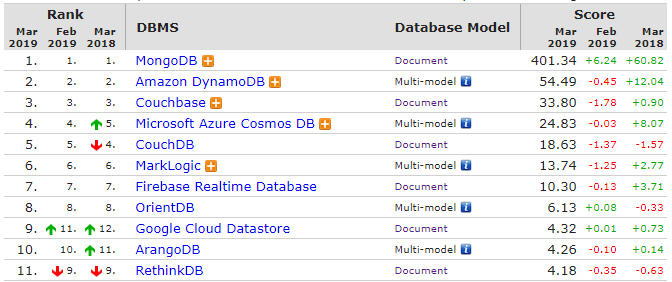
\includegraphics[width=\textwidth]{img/dbRanked.png}
    \caption{Ranking of documented oriented databases}
    \label{docoriented:figure:Ranking}
\end{figure}
Overall not many changes happened in the ranking over that last three years. The development and establishment of these databases can therefore be seen as a longer running process. Three years is a short time frame to retrace the whole market development. To demonstrate how the top 5 as well as RethinkDB (currently 11) established themselves over a longer period consider \autoref{docoriented:figure:Development}. It provides insight in the development of the document oriented database market and the popularity of the leading five products in ranking since 2013 \parencite{dbEngineRankingPopularity}. 

\begin{figure}
    \centering
    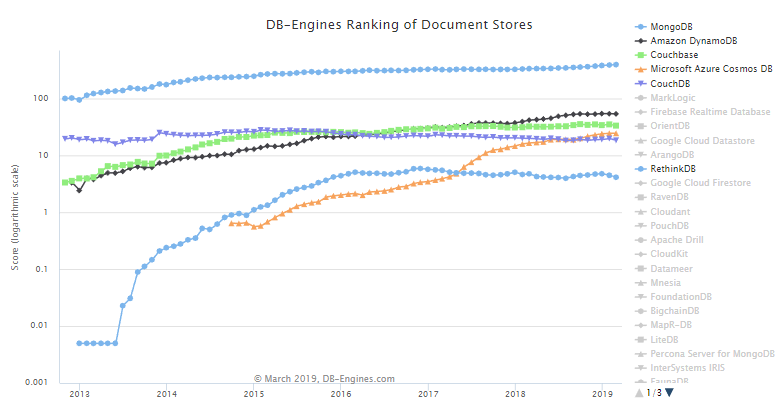
\includegraphics[width=\textwidth]{img/dbRankedTrend.png}
    \caption{Development of the document oriented database market}
    \label{docoriented:figure:Development}
\end{figure}

Ever since 2013 MongoDB has had a leading role. However, the top 3 of today were not as set back then. Further \autoref{docoriented:figure:Development} finally provides a bit more insight over the development of several products over time. CouchDB especially, once second to MongoDB, moved down to rank 5, while Amazon DynamoDB made a name for itself and claimed that second rank. Even though RethinkDB was recently overtaken by Microsoft Azure Cosmos DB it has an astonishing increase in popularity considering its small beginning back in 2013. So in the long run things weren't as set as they have been over the last three years. The historic development of the products and especially the features added, which lead to a sometimes rather steep ascend in popularity, are relevant still.

\subsection{Comparison relational database management systems (RDMS)}
\label{docoriented:section:postalcodes}
Before going into details of specific document store databases this chapter will focus on comparing classical relational database management systems (RDMS) with the new concept of document store databases. This will provide a closer insight into the structure and working of document store databases as well as its general advantages and disadvantages not only in direct comparison.

As the name suggests RDMS focus primarily on relationships. Properties of a data set are spread across different tables and linked using primary and foreign keys to reference and link information. This means a reference - mostly given as a foreign key pointing to the primary key of the needed information entry - can be reused multiple times in different tables across the database. Master data may be used and reused as often as needed, a simple example of a list providing such master data would be a list hosting all relevant postal codes for an application dealing with addresses or shipping in an area. This also means that the data related to a set is spread across the database, needing to be retrieved via the foreign key from different tables. To go over the main differences between such a table and relationship based setup and the document oriented approach, consider the following points.
\subsubsection{Tables}
For RDMS tables are in the centre of the system. Different tables may be linked to describe relationships and reference data. Strictly speaking a single record is described as a row in a table, additional information may be supplied from a different table. All records are bound to this static structure and the columns given in this record table. Therefore records of the same table need to share the same columns to describe their properties.

In the document store based system a single document describes all data related to this entry. No reference to other documents are necessarily made. Seeing that a document always has an unique key to identify it, relations can be technically set up.

Depending on the focus, either the data as such or the common relationships data entries have, a document store or a RDMS brings advantages. It is far easier to group entries in a table sorting by a foreign key reference to for example collect all entries linked to a specific postal code. It is however easier using a document store database to store data which not necessarily shares the exact same properties, therefore cannot be mapped into a strict column based format.
\subsubsection{Schemas}
As the table based design suggests the RDMS is very strict. The schema how columns are used to describe an entry and what data needs to be gathered from another table must be known from the beginning. There is no flexible adaptation depending on the data provided. A record either has all the properties asked for by the schema or null values may be inserted, leading to the question whether the information was unknown, missing or not provided due to an error.

The document store based system can manage documents that differ. This means two entries do not necessarily have to have the same structure or even data attributes \parencite{amazonNoSql}\parencite{objelean}. A common example is a web form where a user can provide some of their details optionally. A RDMS entry would have columns for every property, leaving fields empty if the information is not provided. A document on the other hand stores only the information given.

Advantages depend on the use case scenario. In some cases, especially towards the end of development when a fixed data schema has been agreed on, the very conventional approach of using a SQL database may work just fine. However, especially during development of an application, when data processed is still being explored and especially the difference of data sets (objects) is key to understanding it, a document store may offer more flexibility.
\subsubsection{Scalability}
Relationship databases scale well vertically, the addition of memory or storage to the machine increases the performance. However vertical scaling has a limit, which leads to the need to scale horizontally to further increase performance. The horizontal implementation of RDMS is a complex process that asks for redundancy and different strategies to keep data across the horizontal landscape consistent.

A document based system is much easier to spread horizontally \parencite{ian2016}\parencite{objelean}. Each entry is in itself complete and can be stored across a large landscape since no additional information is linked or needs to be gathered from a possible far away source. The process of storing data across such a landscape is called \enquote{sharding} \parencite{ian2016}.
\subsubsection{Relationships}
Relationships are the central idea of RDMS while tables are the central storage form to implement them. The idea is to associate data entries with different ones to capture relationships and common links. Again, remember the example of the reusable postal code column from section \ref{docoriented:section:postalcodes}.

A document store based system does not provide means to implement this idea. Here the central idea is to keep all data together that is needed to describe a record. If relations are indeed still needed, this needs to happen at application level \parencite{ian2016} using the unique keys that identify the documents (records).
\subsubsection{Querying}
Relational databases tend to use SQL (structured query language) to query their tables and records. Document store databases may support SQL statements, but most are queried with different languages \textquote[\parencite{ian2016}]{such as XQuery, XSLT, SPARQL, Java, JavaScript, Python}  for example.

There are no strict advantages over what query language is being used. However, one might consider the general performance of retrieving records from the database or the complexity of the query statements needed to do common actions (read, write, update, delete) against the specific database with its specific query language.

\section{Couchbase}
\chapterauthor{Andreas Fuchs, Alex Schäfer, Cathleen Schmalfuß}
Some of the general key properties of Couchbase, a document store database, are briefly outlined in the introduction. Later sections will take a closer look at specific characteristics and properties. The context of the CAP theorem will be addressed, as well as relevant characteristics and how they are realized in Couchbase Server. Overall this chapter will give the reader a closer understanding of the ideas behind Couchbase. A short paragraph on the history will provide some insight in the development of this NoSQL database. To cross reference the development steps with the increase of popularity of Couchbase, see \autoref{docoriented:figure:Development} from this chapter’s introduction.

As a document store database Couchbase uses JSON documents to represent data as items \parencite{couchbaseAbout} \parencite{objelean}. As a common way to represent objects, especially in web development, the JSON format makes it easy to store and load data from a Couchbase database. The exact mechanics behind the data structures and the inclusion in buckets will be discussed as part of the core components in section \ref{couchbase:section:corecomponents}.

Couchbase SDKs are available for most common programming languages (e.g. Java, .NET, Node.js, Python and more) and can be downloaded through the package management system of the respective development environment (e.g. Maven, Nuget, npm, pip and more) \parencite{couchbaseWeb} \parencite{objelean}. Thereby a widespread support is given. More information on SDKs and the usage follows in section \ref{couchbase:section:SDK} of this chapter.
Other core characteristics of the Couchbase DB are: its memory-first architecture, an elastic scalability and an architecture based on buckets (which add redundancy and thereby persistence) \parencite{couchbaseWeb}. The core components as well as the architecture itself will be described more closely in the following sections.

\subsection{Couchbase History}
Couchbase DB is a NoSQL document store database that originated in the merge of Membase and CouchOne back in 2011 \parencite{couchbaseWeb}. Membase was build for applications that did not need SQL necessarily, but the durability, replication and data management that RDMS usually provide \parencite{ingenthron}. In the beginning the durability was achieved by MySQL in the background, storing memcached information on disk \parencite{popescuBacalu}. After the merge of CouchDB this responsibility was given to CouchDB implementation, resulting in a new product: Couchbase.

It started out as a \textquote[\parencite{couchbaseAbout}]{pure key-value database}  till it 2012 became a JSON document-oriented database. 2015 SQL-like queries were introduced as well as multidimensional scaling \parencite{couchbaseAbout}. Ever since then, the database was adapted and extended, introducing features like Full-Text search (2017) and Analytics (2018) \parencite{couchbaseAbout}.

\subsection{Architecture}
Before looking at the core components of Couchbase let us take a quick overview of the basic concept behind the architecture of Couchbase and what makes it distinct from other databases.

\begin{figure}[H]
    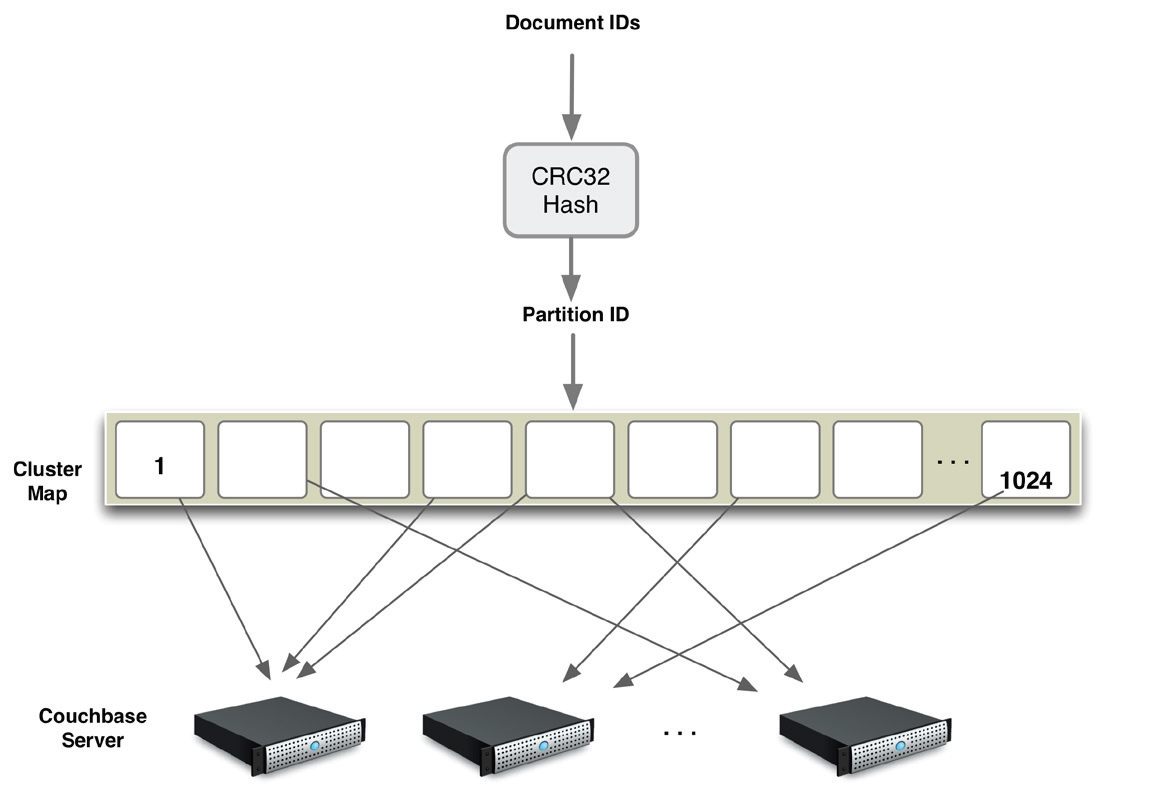
\includegraphics[width=\textwidth]{img/couchbaseClusterMap.jpg}
    \caption{Couchbase's sharding Architecture across its Cluster Nodes}
    \label{couchbase:figure:Architecture}
\end{figure}

Couchbase was designed with a highly distributed architecture from the ground up, which makes it similar to other NoSQL databases. While it could be used on a single machine, the typical setting for Couchbase is a server cluster.
In this environment the data is stored by sharding it evenly across multiple machines. The system defines exactly 1024 partitions (not configurable) and (evenly) assigns them to the available nodes in the cluster. Once a document needs to be stored, the documentId - which is a unique identifier for every document - gets hashed to determine which of the partitions the data is assigned to. \autoref{couchbase:figure:Architecture} illustrates this sharding process. Once the data is assigned, the document will be held in that partition. If nodes are added or removed from the cluster, Couchbase will reassign the partitions among all the nodes to rebalance itself. At any given time the nodes themselves are responsible for their assigned partitions. This leads to another property of Couchbase, which is that all the nodes are completely equal. Every node has two primary processes. The Data Manager is responsible for handling the actual data of the node's partitions while the Cluster Manager deals with the intra-node communication. Those are the reasons why Couchbase is excellent in scaling horizontally. \parencite{objelean}

To make sure that no data is lost when a node has a failure, a replication concept is necessary. Couchbase achieves this by replicating all the partitions and distributing them among the cluster, while making sure that the replica partition is never on the same physical server. This way, once a node fails the cluster will determine the location of the replica and make it the ‘active’ partition.

\subsection{Core Components}
\label{couchbase:section:corecomponents}
This section will focus on some core components of CouchbaseDB. It will provide insight into the mechanics of the database and how the document based database concepts are implemented. To do so the low level concepts of buckets, data schemas and data limits are discussed. This will be the first step to understand availability, scaling and performance of a Couchbase Server infrastructure.
\subsubsection{Keys and Metadata}
The items, stored in documents, are made of keys and values \parencite{couchbaseDocuData}, where a key must be unique within the bucket. In case of nested objects (or attributes) the value can be regarded as an \textquote[\parencite{couchbaseDocuData}]{embedded document}, consisting of key-value pairs or further nested documents \parencite{couchbaseDocuData}. 
Along with the data itself metadata is stored by the server \parencite{couchbaseDocuData} \parencite{objelean} or in case of extended attributes possibly by the application \parencite{couchbaseDocuData}. The server metadata contains a unique ID, a revision or sequence number, an expiration time, flags and the document type\parencite{couchbaseDocuData}. The unique ID, also often simply called key, has the same purpose as the primary key in SQL. The revision or sequence number helps identify the number of mutations of a document, in case of update conflicts this helps find the newest or most current version of a document. The expiration time gives the document a time to live (TTL). This may be either set on document level or bucket level \parencite{couchbaseDocuMemory}. It uniquely identifies any document within the bucket. If the expiration times differ, the bucket TTL \enquote{wins} if the item TTL is longer. If it is shorter, the bucket TTL is left unchanged. Documents without a TTL are automatically given the bucket TTL if it is set \parencite{couchbaseDocuExpiration}. Flags and type metadata are used to identify the type of data as well as the type of the saved value. Extended attributes can either be system set or application set. Server internal extended metadata can \textquote[\parencite{couchbaseDocuData}]{optionally be written and read by user applications}, extended attributes set by the application however can only be accessed by the application which created it \parencite{couchbaseDocuExtendedAttributes}. All server internal metadata is kept in RAM, which leads to \textquote[\parencite{couchbaseWeb}]{100\% memory resident indexes} and provides extremely fast loading (performance).

There are some size limits for the documentId (\enquote{key}), the data (\enquote{values}) and the metadata. The key size is limited to 250 bytes. The value plus the user extended attributes together can not extend 20 MiB. The system extended attributes have a maximum size of 1 MiB. Other fixed metadata such as the id, rev, expiration, flags and type have no limitation \parencite{couchbaseDocuData}.
\subsubsection{Document Store}
Documents in Couchbase DB are stored in JSON \parencite{objelean} or binary format \parencite{couchbaseDocuData}. Any document can be accessed using its unique key. JSON documents can further be parsed, indexed and queried. Binary format can only be retrieved by its key \parencite{couchbaseDocuData}. The general advantage of storing data in document form has already been discussed. In comparison to RDMS, object schemas used in an application can be applied directly as the schema for the document in the database.

This structure also \textquote[\parencite{objelean}]{allows that data [can] be indexed and queried using views}. Entries can be found using a JavaScript-based query engine which is provided by Couchbase Server. There are two main document design approaches to be considered. The first approach is storing a small number of rich documents. This leads to \enquote{fewer relations between independent objects} \parencite{couchbaseDocuDataModel} which in turn increases scalability. Also it is possible to group properties, typically accessed at the same time, increasing atomicity of operations. This is always a good idea since Couchbase guarantees that the ACID fundamentals are given for \enquote{all operations that address a single document} \parencite{couchbaseDocuDataModel}. The other design approach may be a large number of simple documents which possibly hold relations to each other. This is only feasible if the access-pattern is predictable and for some reason (e.g. network speed) the data-size has to be kept small.

The data model of Couchbase holds several advantages. For instance scalability is increased since replications and edits do not affect other documents other than the one replicated/ edited. There is no need to access or touch anything else in the database. Also the latency is kept low since no complex inter-node coordination has to be performed and all connections are minimized \parencite{couchbaseDocuDataModel}. The performance of Couchbase is further increased by the Sub Document API which lets the user access only parts of the inner components of a JSON document. The special Sub Doucment API can run a query against a specific path to either read or write (update) the attribute or document there \parencite{couchbaseDocuSubDoc}. The API was first introduced for Couchbase Server 4.5 and has been available all the way to the current version 6.0 \parencite{couchbaseDocuSubDoc}.
\subsubsection{Data Buckets}
To keep connected data records together, Couchbase Server implements buckets. Buckets are \textquote[\parencite{objelean}]{isolated, virtual containers}. On creation, they are assigned an innumerable name by which the bucket is accessed in the future \parencite{couchbaseDocuBuckMemStor}. No item can be saved before a bucket exists for it \parencite{couchbaseDocuMemory}. Buckets can be replicated leading to redundancy and failure copies \parencite{couchbaseWeb}. There are three types of buckets provided, differing in their way of storing data: Couchbase buckets, Ephemeral buckets and Memcached buckets \parencite{couchbaseDocuMemory}. 

Couchbase Buckets store data both persistently on disk and in memory. High availability is given since data is automatically replicated using the Database Change Protocol (DCP) and scalability accomplished through Cross Data Center Replication (XDCR) \enquote{dynamically scaled across multiple clusters} \parencite{couchbaseDocuBuckets}. If the memory capacity to store data there runs out there are two strategies to eject items from memory. Either value-only, meaning only the value is ejected and the key and metadata kept in RAM, or a full removal strategy. Value-only provides less freed room in memory but will keep up good performance since data can easily be accessed on disk by its unique key. A full removal will lead to more freed memory but less performance since the disk needs to be queried for every request \parencite{couchbaseDocuBuckets}.

Ephemeral buckets are used when persistence is not required. Data is only kept in memory, leading to a highly-consistent in-memory performance. This can be seen especially in case of a rebalance (when a node is added or removed and the system needs to redistribute) and on restart \parencite{couchbaseDocuBuckets}. If this bucket runs out of available memory there are again two strategies: Either it is generally forbidden to add more data than there is room available, which leads to a fail or data is ejected, which leads to a data loss since no data is saved persistently on disk \parencite{couchbaseDocuBuckets}. 

Memcached Buckets cache frequently used data and thereby reduce the number of queries. They provide a directly addressable, distributed, in memory key-value cache \parencite{couchbaseDocuBuckets}. As in-memory suggests, no data is stored on any disk, everything is kept in RAM. If the RAM quota is exceeded data will be ejected and lost.

Couchbase and Ephemeral Buckets are the most commonly used, they \enquote{both provide a highly available, dynamically reconfigurable, distributed data-store} \parencite{couchbaseDocuBuckets}. Persistence for Couchbase Buckets is achieved asychronously between memory and disk. Ephemeral Buckets are only persistent in RAM. Replication, using both DCP and XDCR, is both in Couchbase Buckets and Ephemeral Buckets configurable over a number of servers. For Couchbase Buckets a host server failure leads to the promotion of the replica server which guarantees high availability. For Ephemeral Buckets, the ones which eject data are not permitted to do XDCR though they can be the target of XDCR operations \parencite{couchbaseDocuBuckets}. Rebalance is handled in the same way for Couchbase and Ephemeral Buckets. As buckets and nodes are dynamically added or removed, the buckets and data are distributed evenly across all available nodes \parencite{couchbaseDocuBuckets}.

To increase performance further there are three modes of compression available for Couchbase Sever and data passed through it. This leads to more efficient RAM and disk space usage, reduced need of network bandwidth and higher consumption of CPU \parencite{couchbaseDocuCompression}. Compression is provided by the open-source library \enquote{Sappy} and is works specific to the clients capabilities. The compression mode can be established by the user per bucket \parencite{couchbaseDocuCompression}. The available modes are: off, passive and active.

Off is recommend for clients which will not benefit from compression and if bandwidth usage is no issue. If data is received compressed it will be decompressed to be stored in memory and recompressed to be stored on disk. It is always returned in uncompressed form. Memcached buckets only operate on this mode\parencite{couchbaseDocuCompression}.

the passive mode stores data compressed both in memory and on disk. Data is returned uncompressed unless requested otherwise. Then, data can be returned compressed as well. It is the job of the client to know if it can process compressed data and request accordingly. If uncompressed data is received however, it will only be compressed for disk storage, not in memory. It is then returned uncompressed as well. Advantage of this mode are the reduced memory usage and bandwidth and the reduced CPU usage for the clients that do not required a compressed format \parencite{couchbaseDocuCompression}.

Active mode stores data compressed in memory and on disk no matter what the client handed in. If a client does not support receiving compressed format, it is decompressed before sending it out. This maximizes memory space and network usage. At the cost of wasting CPU time on compression for a client that will need decompressed data as return data \parencite{couchbaseDocuCompression}.
\subsubsection{VBuckets}
vBuckets, sometimes called \enquote{shards}, are \enquote{defined as owner of a subset of the key space of a Couchbase cluster} \parencite{objelean} \parencite{couchbaseDocuVbuckets}. They are used to implement both Couchbase and Ephermal buckets \parencite{couchbaseDocuVbuckets} and have organizational functions such as the distribution of data and replication on more than one node \parencite{objelean} \parencite{couchbaseDocuVbuckets}. Replications are distributed across the cluster. Write operations can only be performed on active buckets, read requests are mostly performed on the active vBucket \parencite{couchbaseDocuVbuckets}. Per bucket, 1024 vBuckets (or 64 on MacOS) are created \parencite{couchbaseDocuVbuckets}. In case of a replication of said bucket all 1024 (or 64) vBuckets are copied \parencite{couchbaseDocuVbuckets}, leading to 2048 vBuckets stored.  Data items are stored evenly across all vBuckets.

To locate and access an item the document key is consulted. The documents all have unique identifiers (the key), which are associated with a specific vBucket using a hashing function mapping \parencite{objelean} (a CRC32 hashing algorithm \parencite{couchbaseDocuVbuckets}). Using this algorithm and the id, the bucket number can be calculated. This number is used to to find the server that \enquote{hosts} the vBucket using a map to determine the correct server node \parencite{couchbaseDocuVbuckets}. The mapping of vBucket to individual node is handled by the Cluster Manager \parencite{couchbaseDocuVbuckets}. After the node has been identified the operation can be performed directly on this server node.

In case of a cluster-configuration change (addition or removal of nodes) first the replica buckets are promoted if applicable. It is applicable in case the active buckets are lost due to a failure or deletion. After that, primary and replica buckets are redistributed across the newly available buckets. Last the Cluster Manager updates the mapping and sends it out to all cluster-partitions \parencite{couchbaseDocuVbuckets}.

\subsection{Querying}
\subsubsection{N1QL} \label{couchbase:n1ql}
Couchbase has its own query language called N1QL (pronounced \enquote{nickel}) \parencite{couchbaseDocN1Ql}. Even though Couchbase Server is a NoSQL database, N1QL is very similar to SQL in syntax and use. However, as the information can be nested within documents N1QL features some additions that are not needed in SQL. The basic clauses in N1QL are: 
\begin{itemize}
    \item SELECT
    \item FROM
    \item LET
    \item WHERE
    \item GROUP BY
    \item ORDER BY
    \item LIMIT
    \item OFFSET
\end{itemize}
The expression used in a SELECT statement can be either literal values, calculations or properties from documents. If the properties are specified in the statement, the result will contain only the given properties from matching documents. It is possible to use a wildcard selector (*), in which case the query returns each matching document in its entirety. The id that is assigned to each document by Couchbase Server is not included when retrieving the complete document. To get this information, the META() function needs to be utilized. It returns a document that contains metadata about the document it belongs to. Its properties like the documentId can be accessed via a \enquote{dot} notation: META().id \parencite{proCouchbaseServer}.

The FROM statement is where the source to retrieve data from is defined. In SQL this is the name of the database. Similarly, in N1QL the name of the bucket to search in is given. However, this is not the only type of source that can be stated. It is possible to query only from certain properties (or even properties of properties) if necessary. Again, this utilizes the simple \enquote{dot} notation  \parencite{proCouchbaseServer}. An example of this would be: \texttt{SELECT * FROM userdata.user.role}. This query retrieves all properties from the role property of the user property from documents in the userdata bucket. This allows developers to build more flexible queries when dealing with heavily nested structures. Another option to define the source is to use a subquery. This means that within the FROM clause, another query is being executed, the result of which is used as the source for the outer query \parencite{couchbaseDocN1Ql}. Just like in SQL, N1QL allows for joins of different sources. The JOIN ... ON KEYS clause, which is used to execute joins, takes a property from one bucket which is then used as a key in another bucket. For example \texttt{SELECT * FROM books AS b JOIN authors AS a ON KEYS b.author;} returns all documents from the \enquote{books} bucket with additional info from the \enquote{authors} bucket, looked up in authors with author property in books.

The LET statement makes it possible to define variables to use in other parts of the query. The value of a variable can be the result of a subquery. The WHERE clause allows for filtering of documents for specific characteristics. In it, developers can execute calculations and create boolean expressions by comparing values or combining boolean values with AND or OR clauses \parencite{couchbaseDocN1Ql}. To group resulting documents together, the GROUP BY clause is used. Given a property, it aggregates certain values according to the property. The ORDER BY clause orders the results by a given property \parencite{proCouchbaseServer}. To reduce the number of documents shown in the result, a maximum number can be set using the LIMIT clause. The given number corresponds to the amount of result documents. The OFFSET clause is used to not start with the first document, but with a later one. If the Limit is 1 and the Offset is 1 as well, only the second document from the entire result will be returned \parencite{proCouchbaseDev}.
\subsubsection{Views}
Couchbase offers another way to retrieve data: views. They allow developers to create more complex queries by writing their own functions and perform calculations on the data in the same step. Views use the MapReduce programming model to enable them to process documents across a cluster. For each view a map function is defined, which is applied to every document in the bucket and takes care of the initial filtering and processing of the documents \parencite{proCouchbaseServer}. The result of the map function is an index, which is a list of key-value pairs. This index is then stored on the disk and is updated when the documents change \parencite{couchbaseDocViews}. Each view can also have a reduce function, which performs aggregations on the data. Couchbase Server provides commonly used reduce functions (e.g. basic statistical functions) \parencite{proCouchbaseServer}. Once the map and reduce functions are defined, the view can be queried. Every time a view is queried, Couchbase Server builds a new index by default, to make sure that all changes that were made since the last query are in the index. As building an index takes up a lot of resources, developers can decide depending on their application wether or not a new index should be built for every view queried \parencite{couchbaseDocViews}.


\subsection{Performance}
When deciding which database to use for an application, it is important to consider its performance under high load. The instantiation of a Couchbase bucket is faster than of an SQL database, but slower than other NoSQL databases. When tasked with executing a large number of reading operations, Couchbase proves to be more efficient than other databases, handling even large amounts of operations very fast. The same result applies to delete operations \parencite{compNoSQLandSQL}.  As for loading data into the database, Tang and Fan (\parencite{insert}) showed that Couchbase performed inserts faster than Cassandra and HBase, but slightly slower than Redis and MongoDB. Additionally, they state that the performance decreases in comparison to other NoSQL databases with an increasing number of documents to be inserted.


\subsection{Monitoring}
To setup and maintain your Couchbase database, the Couchbase Web Administration Console offers a lot of information and direct interaction with your database. Part of that is the monitoring section, which provides details on resources used by the cluster, each node or bucket. The level of detail one wishes to see is adjustable. Additionally, the Web Administration Console not only shows numbers, but visualizes them as graphs so they are easier to grasp \parencite{getStarted}. The overview of the entire cluster shows information on resource usage across buckets, e.g. RAM available for the cluster, RAM used by buckets and RAM allocated by buckets. Similar information is given for the disk space that is used. In addition, graphs provide insight about the operations and disk fetches per second, which are valuable to keep an eye on the overall condition of the database and the application it is used for. \parencite{proCouchbaseServer}.

\begin{figure}
    \centering
    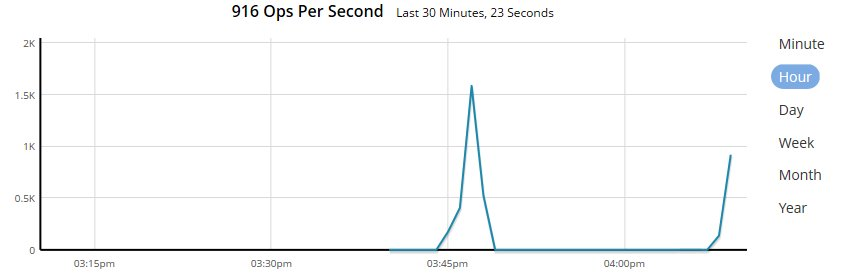
\includegraphics[width=\textwidth]{img/couchbaseMonitorOps.jpg}
    \caption{Monitoring the operations per second}
    \label{couchbase:figure:ops}
\end{figure}

\autoref{couchbase:figure:ops} shows two spikes in operations per second in the last hour, which timestamps correspond to the queries executed before.

\begin{figure}[H]
    \centering
    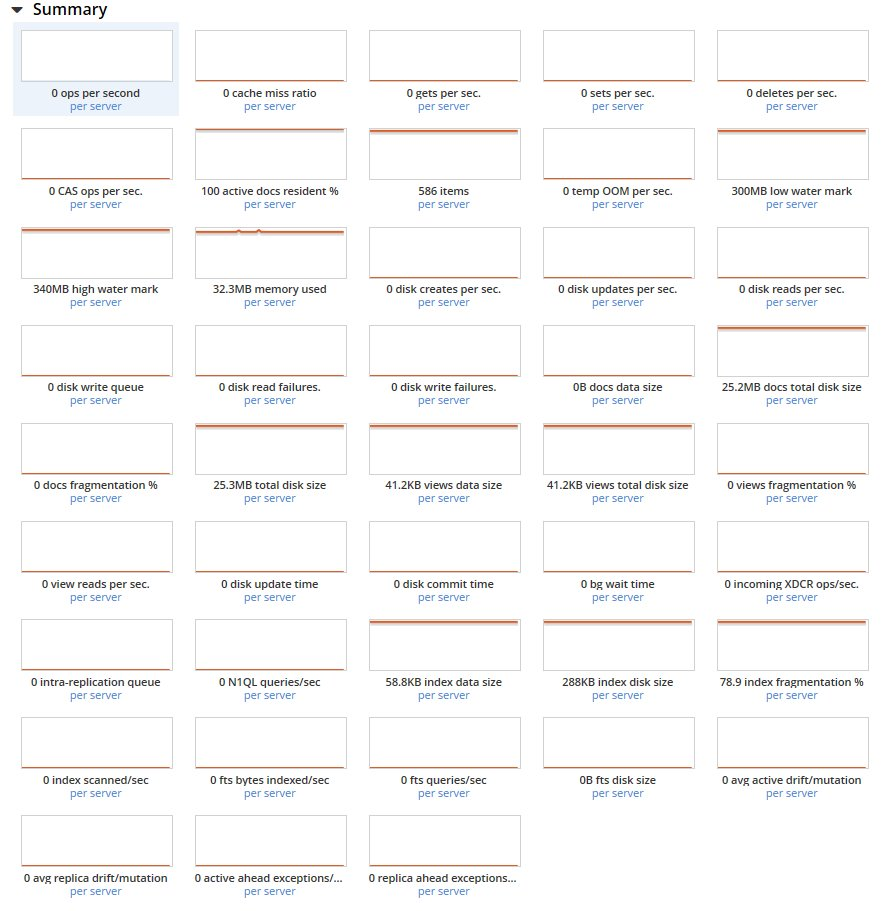
\includegraphics[width=\textwidth]{img/couchbaseMonitor.jpg}
    \caption{Monitoring metrics of an individual bucket in Couchbase}
    \label{couchbase:figure:Monitoring}
\end{figure}

\autoref{couchbase:figure:Monitoring} shows all the graphs available for individual buckets. All in all, over forty metrics can be viewed and used to assess the health and performance of the system.

\subsection{CAP Theorem}
From a CAP-Theorem perspective Couchbase can be operated as a CP or CA system. By default it will act as CP system. When a Node fails some data will be temporarily unavailable for writes until the replica is set to active. However, reads will be processed regularly by the replicas available in the cluster. If needed, it can be tuned to act as a CA system for example through auto-failover. But this is only half the story and only applies if Couchbase is run in a single cluster setting. With a multiple cluster setting, also known as Cross Data Center Replication (XDCR), it will act as AP system. Since in this setting any Cluster can be written to, problems arise when the same data is modified from different locations. In this case Couchbase provides different configurations for conflict resolution (for example through timestamp or revision ID), eventually leading to consistency between multiple clusters. \parencite{couchbaseCAP}

\subsection{SDK}
\label{couchbase:section:SDK}
To use Couchbase productively in a development environment this last section shall discuss the available software development kit and give some examples on how to use it to perform basic \gls{crud} operations on the cluster's data.

First of all, Couchbase offers SDKs for several popular programming languages and runtime environments inlcuding C, Go, Java, .NET, Node.js, PHP and Python. \parencite{couchbaseSDK} Since it would be out of scope to give examples for all of them, this section will limit the examples to the Node.js SDK, but the information given will be easily transferable to other languages as well.

First, a connection to the Couchbase Cluster needs to be established. Afterwards, authentication is necessary to select the desired bucket. Once there is a bucket object it can be used to send queries. The described steps can be seen in Listing \ref{couchbaseAuthAndBucket}.

\begin{listing}[ht]
\begin{minted}{js}
const cluster = new couchbase.Cluster('localhost:8091');
cluster.authenticate('user', 'password');
const bucket = cluster.openBucket('demo-bucket');
\end{minted}
\caption{Connect to Couchbase}
\label{couchbaseAuthAndBucket}
\end{listing}

Two different kinds of interacting with the data shall be looked at. The first option is to use the core operations upsert(docId, document), insert(docId, document), replace(docId, document), get(docId) and remove(docId) to execute the basic \gls{crud} operations. Insert will only insert the document if the docId isn't found, replace will only replace the document if the docId is found and upsert will always replace the document (ignoring if the docId existed or not). The second option is to use N1QL queries described in \autoref{couchbase:n1ql} to query the desired data. Examples for both options can be seen in Listing \ref{couchbaseCRUD} and Listing \ref{couchbaseSDKN1QL}.

\begin{listing}[ht]
\begin{minted}{js}
// Remove and Get use the same syntax
bucket.get('uniqueDocId', function(err, res) {
    if (err) {
        console.log('operation failed', err);
        return;
    }
    
    //res contains the document
    console.log('success!', res);
});

// Replace, Insert and Upsert use the same syntax
bucket.insert('unqiueDocId', {some:'value'}, function(err, res) {
    if (err) {
        console.log('operation failed', err);
        return;
    }

    console.log('success!', res);
});
\end{minted}
\caption{CRUD Operations}
\label{couchbaseCRUD}
\end{listing}

\begin{listing}[ht]
\begin{minted}{js}
const q = couchbase.N1qlQuery.fromString('SELECT airportname as n
    FROM `travel-sample` where type="airport" LIMIT 4');
// Using arrow functions to iterate through the result set
bucket.query(q, (err, rows) => rows.forEach((row) => console.log(row)));
\end{minted}
\caption{Query Data with N1QL}
\label{couchbaseSDKN1QL}
\end{listing}

It is important to note that while in earlier versions of the SDK it was not possible to stream the results of N1QL queries row by row (and instead had to wait for the complete result set) recent versions do not have this limitation anymore.

It should be clear that the presented examples are far from showing all of the offered capabilties of the Couchbase SDK and merely offer an easy introduction. To explore more of its capabilities, like MapReduce Views or Concurrent Document Mutations, the Couchbase Documentation is an excellent place to start.

\subsection{Conclusion}
To sum it all up there are several key takeaways from this research into Couchbase, its mechanics and its take on the CAP theorem. High performance in Couchbase is achieved due to the partitioning into small vBuckets, compressed data transmission and in memory strategies for at least the most important metadata (unique documentId). In terms of the CAP-Theorem the decision whether Couchbase is rather AP (Availability and Partition Tolerance) or CP (Consistency and Partition Tolerance) depends strongly on the cluster setup. What can be said, especially in comparison to relational databases, is that Couchbase (same as most document oriented databases) scales well horizontally. A reason for that is the vBucket partitioning and the equality of nodes.

Use Cases that make Couchbase a good database choice are cases of large amounts of unstructured data. Due to the not fixed schema, Couchbase can work with changing requirements of application object structure or general data schema. Another scenario where Couchbase stands out against other document oriented databases are performance scenarios.

This chapter gave you a broad overview of Couchbase, its components and its classification within the CAP theorem. Other very important aspects of modern databases could not be covered however. The aspects security and user permission management were not discussed and are to be researched further in the future.

\section{RethinkDB}
\chapterauthor{Anne Born, Dorian Czichotzki}

\subsection{Introduction}
In today's data-driven world, the availability of information in real-time becomes more and more important. Many applications rely on an analysis and delivery of data in a time-frame that is considered as immediate by the user. Be it multi-player games, real-time analytics or connected devices in an IoT infrastructure \autocite{Wingerath2017}. Data should not only be delivered quickly but also proactively, focusing more on a push-based architecture, giving the responsibility to keep the client informed to the server, instead of the conventional pull-based database were the client has to request information each time it is of interest.  One kind of technology, implementing this immediate handling of information are so called real-time databases, which are discussed in this chapter by reference to RethinkDB, an example for such a push-based database.
The chapter is structured as follows.


First, an introduction to real-time databases in general is provided and a concrete definition of the term in the context of RethinkDB is given. The following sections then discusses the real-time database RethinkDB in great detail, providing information on the architecture, use-cases it is suited for, and most importantly where the technology could be placed in the CAP-Theorem.

\subsection{Real-time Databases}
\label{sec:rethink_real-time}
Like many terms in the IT, real-time databases have an abundance of different definitions. Some overlapping to a great extend, others having nearly no intersection at all. This makes for a need to introduce some of the most common definitions with the goal of establishing a precise interpretation of the term in the context of this book and - particularly - this chapter.


One of the first indications of the term real-time database was within a special issue of the ACM SIGMOD Record on Real-Time Database Systems in March 1988 \autocite{Eich:1988:44203}. In an article of this journal called "Issues and Approaches to Design of Real-Time Database Systems" Mukesh Singhal defined the use-case for real-time databases as "applications which have severe performance constraints such as fast response time and continued operation in the face of catastrophic failures" \autocite[p.  1]{Singhal:1988:IAD:44203.44205}. He further mentions timing constraints as a direct derivation of the use-cases mentioned above, laying a fundamental basis for one of the most common definitions of said technology.


This definition (referring to real-time databases as databases that fulfil time-constraints and must meet certain deadlines), also probably the most popular one, is not the one used in the context of RethinkDB.


Instead, the definition used in this book is based on a medium article by Wolfram Wingerath \autocite{Wingerath2017} who claims that "in recent years, people have come to expect reactivity from their applications, i.e. they assume that changes made by other users are immediately reflected in the interfaces they are using" \autocite{Wingerath2017}. From this statement it can already be derived that he defines the use-cases for real-time databases differently from Singhal. Instead of applications that need fast response time for security reasons, like applications for power-plants or hospitals, he defines a general demand for reactive applications for the sole reason of improved user experience. However, similarly to Singhal, Wingerath also sees a need for new technology besides conventional databases. Conventional databases being pull-based applications that only represent the state of the system at a single point in time. As an alternative to those databases he defines real-time databases as technology that facilitates the push-based handling of changes, "taking view maintenance out of the application layer" \autocite{Wingerath2017}. A real-time databases thus must provide some functionality for clients to 'subscribe' to certain events (changes), receiving updates when the event is triggered. This subscription-feature' is what he calls 'real-time queries'.


Real-time queries can fall into one of two different categories:

\begin{itemize}
    \item Self maintaining queries
    \item Event stream queries
\end{itemize}

The former delivers not only the information that something has changed but also the old and new value. This of course only works if the query is executed again each time a change took place. The latter type of queries only provides the information that a change took place without any more details.


Both queries are push based, pushing information to the client.


Summarised, real-time databases, as defined in this book, are databases that facilitate a push-based method instead of only allowing pull-based query execution. This makes the development of reactive applications much more feasible, since it allows for data updates in a publish/subscribe-like manner.

\subsection{RethinkDB}
After giving an introduction to real-time databases as defined in this book, the document-based database RethinkDB is introduced and discussed in great detail. In order to understand not only the database itself but also its place in the CAP-Theorem this chapter is structured in the following sections: Firstly this section will provide an overview over RethinkDB and its core features, next a short section on the history of the database gives some more insight into the story of RethinkDB and its community, then the proprietary query language ReQL is introduced and explained briefly. Finally the architecture that this database is based on is outlined, including the distribution of RethinkDB over multiple nodes, the functioning of query executions and the storing of data.


Most of the information displayed in this chapter is from the official RethinkDB website \autocite{rethinkdb}.\bigskip
RethinkDB defines itself as "the open-source database for the real-time web" \autocite{rethinkdb}.


From this description it is already possible to derive two of the most important features of the database project. The first being that it is 'open-source' meaning that its source code is publicly available\footnote{https://github.com/rethinkdb/rethinkdb}. RethinkDB itself is developed and enhanced by a combination of core team developers and database experts as well as over 100000 other contributors from the RethinkDB community, using the open-source aspect to provide their knowledge to the project.


The second feature that the RethinkDB project uses frequently to describe itself is being a database 'for the real-time web'. This means, that RethinkDB falls exactly in the definition of real-time databases established in \autoref{sec:rethink_real-time}, providing a function called "changefeeds" (see \autoref{sec:rethink_changefeeds}) that is push-based and thus automatically updates the client in case of changes.


This feature is already a pretty unique characteristic of RethinkDB.
Another one is the fact that the ambitious project was written from the ground up in C++, not relying on and extending existing database implementations.
This approach of creating something completely new and \enquote{rethinking} databases also lead to the development of a proprietary querying language, that is discussed in \autoref{sec:rethink_reql}.

\subsubsection{History}
RethinkDB is originally the product of the eponymous company founded in 2009 with the goal to "bring a breath of fresh air to the database world" \autocite{rethinkdb:announcement}. At this point the database was not open-source, but also not released as a production ready version yet. With version 1.2 released in November 2012, the company first decided to open-source their project \autocite{rethinkdb:open_source}.


After three more years of development in 2015, RethinkDB 2.0 was released and with it the first production ready version of the real-time database \autocite{rethinkdb:production_ready}. One year later, however, the company was shut down, terminating the official support for the production versions that was offered until then \autocite{rethinkdb:shutting_down}. In the blog article announcing the shut down of the company, it was also signalised that the RethinkDB team plans on continuing the development of their product with an open-source continuity plan, keeping it available under an open-source license. Due to this continuous effort of former RethinkDB employees and people from the community to "transition it to a community-driven endeavour" \autocite{rethinkdb:linux_foundation}, the source-code was purchased by the Cloud Native Computing Foundation in 2017, who published it under the Apache License 2.0.


As of today the RethinkB project is extended by a large open-source community with version 2.3 being the latest release.

\subsubsection{ReQL}
\label{sec:rethink_reql}

As mentioned previously, one of the main features of RethinkDB is its powerful, proprietary query language called ReQL.
Since this language is the base of all interaction between the client and the server (the database), it will be discussed in detail in the following sections, explaining its core attributes, the supported data-types and providing examples for different functionalities \autocite{rethinkdb_reql}.

\paragraph{Data Types}
To facilitate a deeper understanding of ReQLs mechanics, this section gives an insight into the different data types that are supported by the querying language.
In the official documentation, RethinkDB distinguishes two main categories \autocite{rethinkdb:data_types}:

\begin{itemize}
    \item Basic data types
    \item RethinkDB-specific data types
\end{itemize}

Each of the aforementioned categories is explained briefly.

\subparagraph{Basic data types}
This category includes the data types supported by nearly every programming or query language.

\begin{itemize}
    \item Numbers
    \begin{itemize}
        \item This data type includes any real number. Internally values of this type are represented as double precision floating point numbers. This leads to a size of 64 bits.
        \item allowed (examples): 2, 5.8276, -13.4
        \item not allowed: infinity, NaN
    \end{itemize}
    \item Strings
    \begin{itemize}
        \item The data type of string is used the same way it is commonly used in other query languages as well. The encoding used by ReQL is UTF-8, which is why any valid UTF-8 string is also a valid ReQL string. This includes the usage of the null code point (U+0000).
    \end{itemize}
    \item Booleans
    \begin{itemize}
        \item A boolean can attain the values true or false.
    \end{itemize}
    \item Null
    \begin{itemize}
        \item Nearly every programming language has a data type similar to Null, however the naming may be different from language to language. Since ReQL can be embedded into many different programming languages (see \ref{sec:rethink_reql_features}) it might be called something different from Null (e.g.: nil or none). It is important to mention that Null does not equal the number zero (0), the empty set ({}) or a string with a length of zero (""). Instead Null is used to emphasise the absence of a value. For example the parent of a root node could be Null, since it does not exist.
    \end{itemize}
    \item Objects
    \begin{itemize}
        \item Since RethinkDB belongs to the category of document stores and it more specifically is designed to  store JSON documents, any valid JSON object is also a valid object in ReQL. This includes but is not limited to simple key-value pairs \textit{({name: "Harry Potter"})} or nested objects. 
    \end{itemize}
    \item Arrays
    \begin{itemize}
        \item Equally to the documents mentioned above, the array data type of ReQL is also based on JSON arrays, meaning that any valid JSON array is also a valid ReQL array \textit{([1, 2, 3] [] [{name: 'Harry', age: 23}, {wizard: 'Dumbledore', age: 112}])}. The maximum number of elements inside an array can be changed at runtime, the default, however, is 100000. But RethinkDBs internal handling of arrays makes them inefficient at large sizes
    \end{itemize}
\end{itemize}

\subparagraph{RethinkDB-specific data types}
Data types of this category are specific to the functioning of RethinkDB and ReQL. They are not supposed to be used as actual data but instead are either what RethinkDB uses internally to store data or as return values to queries. An exception to this are the so-called 'pseudo types'. Those can be used as actual data types for values defined by the user, but are specific to RethinkDB in a way that they are not commonly implemented in most programming languages.

\begin{itemize}
    \item Databases
    \begin{itemize}
        \item This data type describes RethinkDB databases. When using the '.db' operation, this is the return value. A database holds tables and administrative information.
    \end{itemize}
    \item Tables
    \begin{itemize}
        \item This data type describes RethinkDB tables. They can be used as selectors. Additionally documents can be added, updated or deleted making tables writable.
    \end{itemize}
    \item Streams
    \begin{itemize}
        \item Similar to the aforementioned arrays, streams are lists. However, in order to make working with large result sets more feasible a Stream is represented by a cursor that points to the result set. This means, that instead of retrieving the entire result at once (like an array) a loop is employed to only retrieve one result set at a time, making it more performant. Another difference between streams and arrays is that the former is read-only and thus can not be changed. This limits the chainability of commands that return a stream.
    \end{itemize}
    \item Selections
    \begin{itemize}
        \item Selections are a subset of the table data type. Many table operations (for example \mintinline{python}{filter} and \mintinline{python}{get}) return a selection. Selections exist as a counterpart to three different data types: \mintinline{python}{Selection<Object>}, \mintinline{python}{Selection<Arrays>} and \mintinline{python}{Selection<Stream>}. Due to the chainability of ReQL commands the Selections are writable and can be passed to other ReQL operations
    \end{itemize}
    \item Pseudotypes
    \begin{itemize}
        \item As mentioned previously the pseudotypes form an exception to the other RethinkDB-specific data types since they can be used with user data similarly to the basic types. Generally they are either special cases of other types or a composition of multiple other types. The pseudotypes include binary objects, times and geometry data types.
    \end{itemize}
\end{itemize}

ReQL provides its users with the 'typeOf' command, returning the data type of operations (see \autoref{lst:rethink_typeOf}).

\begin{listing}[ht]
\begin{minted}[breaklines,breakbefore=.]{python}
r.table('wizards').get(1).typeOf()

# returns:
# "SELECTION<OBJECT>"
\end{minted}
\caption{Usage of the TypeOf command}
\label{lst:rethink_typeOf}
\end{listing}

This short description of the data types supported by ReQL already gives an insight to all the possibilities of querying with RethinkDBs proprietary query language. The following sections will extend this insight by introducing some of the many features that ReQL provides.

\paragraph{Features}
\label{sec:rethink_reql_features}

ReQL itself is designed to offer an extensive amount of functionality, enabling users to not only manipulate json documents but also facilitating the usage of common \gls{sql} capabilities. To achieve this ambitious goal the language is based on functional programming languages like Haskell and Lips. However, a knowledge of those languages is not necessary, since ReQL was developed to embed into an abundance of different programming languages. To allow for this natural integration into different languages so called 'drivers' are developed. The official RethinkDB Website groups the existing drivers into three categories:

\begin{enumerate}
    \item Official Drivers
    \begin{itemize}
        \item Drivers developed and maintained by the core team of RethinkDB developers
    \end{itemize}
    \item Community-supported drivers
    \begin{itemize}
        \item Drivers developed and maintained by members of the large open-source community of RethinkDB. To be accepted as a community-supported driver, the json driver protocol has to be used and the features of at least Rethink 2.0 ReQL must be supported.
    \end{itemize}
    \item Drivers with limited features
    \begin{itemize}
        \item Drivers developed by members of the open-source RethinkDB community, that do not provide full support of RethinDB 2.0 ReQL.
    \end{itemize}
\end{enumerate}

A list with all available drivers by category (as of April 2019) can be found in \autoref{appendix:rethinkdb:listofdrivers}.
To use ReQL in one of the (partially) supported programming languages the user must import the driver the way that is specified by said programming language. Afterwards he/she can construct queries by calling methods from the driver.


Listing \autoref{lst:rethink_python_import} shows how this works exemplarily for python. 

\begin{listing}[ht]
\begin{minted}{python}
#import the RethinkDB package
import rethinkdb as r  
#connect to the server on localhost and default port
conn = r.connect()       
#create a table `users`
r.table_create('users').run(conn)  
#get an iterable cursor to the `users` table
r.table("users").run(conn)          
\end{minted}
\caption{Importing ReQL as a package to python}
\label{lst:rethink_python_import}
\end{listing}

 Of course this embedding of ReQL has limitations. One can not use every feature offered by the 'host language'. This applies to those operations, that have side effects and control blocks. Listing \autoref{lst:rethink_side_effects} shows the limitations of embedding ReQL with the help of an example. It illustrates two ways of getting all documents that match certain criteria, one employing operations native to python (if - else) and one employing the 'r.branch' command included in the RethinkDB package.


In this listing only the latter query would work, since the first one is based on python operations with side effects. Other operations and control blocks that can not be used inside ReQL queries include but are not limited to print statements, switch-case statements and loops.

\begin{listing}[ht]
\begin{minted}[breaklines,breakbefore=.]{python}
# WRONG: Get all wizards older than 30 using the `if` statement
r.db("wizards_world").table('wizards').filter(lambda wizard:
    True if wizard['age'] > 30 else False)

# RIGHT: Get all wizards older than 30 using the `r.branch` command
r.db("wizards_world").table('wizards').filter(lambda wizard:
    r.branch(wizard['age'] > 30, True, False))
\end{minted}
\caption{Limitations of the embedding of ReQL}
\label{lst:rethink_side_effects}
\end{listing}

Additionally, this listing also gives an insight into another important functionality of ReQL: Chaining commands. To construct a query in this query language, a nearly arbitrary number of commands can be chained together, separated with '.'.


To emphasise on this feature and to really illustrate how it works, listing \autoref{lst:rethink_chaining} provides a good example for this. First, all documents of a specific table are returned, then by adding '.pluck("last\_name")' only the last\_name field of each document is returned. This can then be filtered further by adding '.distinct()' to it and so forth.
\begin{listing}[ht]
\begin{minted}[breaklines,breakbefore=.]{python}
# Get all entries of a table
r.db("wizard_world").table("wizards")

# Return only the last names of the documents
r.db("wizards_world").table("wizards").pluck("last_name")

# Get all the distinct last names (remove duplicates)
r.db("wizards_world").table("wizards").pluck("last_name").distinct()

# Count the number of distinct last names
r.db("wizard_world").table("wizards").pluck("last_name").distinct().count()
\end{minted}
\caption{Chaining of commands in ReQL}
\label{lst:rethink_chaining}
\end{listing}

As previously mentioned ReQL has many powerful features, including the \gls{sql}-like combination of multiple tables with JOINs. For reasons of performance JOINs in ReQL are automatically distributed (see \nameref{sec:rethink_arch_query_execution}).


Now anyone who is familiar with \gls{sql} knows that many different JOINs exist in the world of databases. RethinkDB supports four, called inner-join, outer-join, eq-join and zip. The first two work similar to their \gls{sql}-counterparts, which is why they are not discussed in greater detail in this book. The last and second last however, are ReQL specific and will be explained with the help of a short example.

\begin{listing}[H]
\begin{minted}[breaklines,breakbefore=.]{python}
r.db("demo").table("wizards").eqJoin("house", r.db("demo").table("houses"))
# Example output only eq_join (one document)
\end{minted}
\begin{minted}[breaklines,breakbefore=.]{json}
{

    "left": {
        "haircolor": "brown" ,
        "hobbies": "Collecting magical creatures" ,
        "house": "d20dda48-6112-499b-ac2f-5288faa6bb4f" ,
        "id": "a7892a90-a211-493a-a194-734d12387741" ,
        "name": "Newt Scamander"
    } ,
    "right": {
        "animal": "badger" ,
        "house": "Hufflepuff" ,
        "id": "d20dda48-6112-499b-ac2f-5288faa6bb4f" ,
        "score": 60
    }

} 
\end{minted}
\caption{The Eq-Join function in ReQL}
\label{lst:rethink_eq_join}
\end{listing}
\begin{listing}[H]
\begin{minted}[breaklines,breakbefore=.]{python}

r.db("demo").table("wizards").eqJoin("house", r.db("demo").table("houses")).zip()
#Example output with zip() (one document)
\end{minted}
\begin{minted}[breaklines,breakbefore=.]{json}
{

    "animal": "badger" ,
    "haircolor": "brown" ,
    "hobbies": "Collecting magical creatures" ,
    "house": "Hufflepuff" ,
    "id": "d20dda48-6112-499b-ac2f-5288faa6bb4f" ,
    "name": "Newt Scamander" ,
    "score": 60

} 
\end{minted}
\caption{The Zip function in ReQL}
\label{lst:rethink_zip}
\end{listing}

The 'eq\_join', as any other join, has the goal of combining two tables with the help of a common indicator. In this case, a function can be applied to any field of the left-hand table and is then matched to the right-hand tables primary keys or secondary indexes. Since ReQL automatically adds a primary key for each document in a table, users have the option of declaring other fields as secondary indexes if needed, speeding up many read queries \autocite{rethinkdb:secondary_indices}.
The 'eq\_join' command is more performant than the inner or outer join and operates more efficient.


Considering listings \autoref{lst:rethink_eq_join} and \autoref{lst:rethink_zip} one can not only see an example of an eq\_join query, but also an example output. This output of course only displays one entry of an array of documents that are returned as a result of this query. When taking a look at the first query of this listing, it becomes apparent, that the output is split into a left and right side. Each side contains the matching document of the respective table.


The second query of the listing \autoref{lst:rethink_eq_join} shows how the two 
parts can be merged together with help of the zip function. This function is "used to 'zip' up the results of a join by merging the 'right' fields into 'left' fields of each member of the sequence" \autocite{rethinkdb:zip}.


Of course, it is way out of scope for this chapter to provide a comprehensive guide on all of ReQLs many functions and features. However, RethinkDB has an extensive and well-written documentation, enabling users of all skill levels to write ReQL queries \footnote{https://www.rethinkdb.com/docs/}

\subsubsection{Architecture}

RethinkDB is supposed to be used in a cluster configuration. Despite the database being capable of running on a single server, many of the replication features, described below, will only be available in a cluster. The Raft algorithm is used to distribute cluster configuration between nodes.

\paragraph{Sharding \& Replication}

Data is partitioned into shards (see \cite{rethinkdb:architecture}). Each table in the database can have up to 64 shards. When a table gets sharded the data is divided into a specified amount of equally sized ranges. The primary key of each document determines the shard a document will be stored in. After shard creation there is no automatic re-balancing mechanism. Therefor re-balancing activities must be initiated manually.


Shards can be replicated over multiple nodes. A set of replicas always has one primary shard. The primary shard is responsible for all write and read operations on the documents it holds. When a table is configured for replication, RethinkDB applies a set of heuristics to distribute the shards over multiple systems. Alternatively the Database can be configured to distribute shards to specific servers in the cluster by facilitating server tags. Server tags are identifiers for one or a set of servers.


\paragraph{Query Execution}
\label{sec:rethink_arch_query_execution}
Query Execution is a multi-step process that can be described as follows.

\begin{enumerate}
    \item One server in the cluster receives a query from a client and creates an execution plan in form of a stack. Lower operations on the stack retrieve data. Higher operations transform the data.
    \item The stack is distributed to every relevant server in the cluster for execution. All participating nodes can operate in parallel and stream their results upwards the execution stack.
    \item The results are aggregated and sent to the client
\end{enumerate}

To enable concurrent access, RethinkDB uses a copy-on-write mechanism for documents that are already read by an other client. A write operation will lead to consistent results just for a read operation that was started after the write process finished completely. If multiple clients try to write to the same document simultaneously, exclusive block-level locks are used. The client does not notice or manually control the lock mechanism.

\subparagraph{Atomicity of operations}
Most operations changing a document are atomic in nature. An update operation can be finished in a single operation as long as the execution is proven to be deterministic. Exceptions in RethinkDB are operations that facilitate JavaScript operations, random values and sub-query execution.

\paragraph{Data Storage}
Data can be stored using many common file systems. The most performant solution is too use direct disk I/O. Data in the system is organised in B-Trees and managed by an integrated storage engine. The engine is capable of automatic garbage compaction and is inspired by \gls{btrfs}.

\subsubsection{Change feeds}
\label{sec:rethink_changefeeds}
The main feature of RethinkDB is to actively push changes to a client, when these occur. In ReQL this behaviour can be triggered by using the \mintinline{js}{changes()} operation in a query\autocite{rethinkdb:changefeeds}.

To receive changes on a table called \textit{Houses}, one can execute the following query:
\mint{js}{r.table("Houses").changes();}

The query would result in a constant stream of changes in the form shown in Listing \autoref{lst:rethink_changefeedresult}. For more efficient use only changes are transmitted.

\begin{listing}[H]
\begin{minted}{json}
{
"new_val": {
    "id":  "0539dcdb-f0f7-482c-9721-ead006dfef30" ,
    "name":  "Gryffindor" ,
    "points": 0
    },
"old_val": {
    "id":  "0539dcdb-f0f7-482c-9721-ead006dfef30" ,
    "name":  "Gryffindor" ,
    "points": 202
    }
}
\end{minted}
\caption{Form of a single change response}
\label{lst:rethink_changefeedresult}
\end{listing}

The change feed feature can be used with many different other features of the query language and does not have to be applied to the end of the query all the time. The next example plucks the output of the change feed to only show the \textit{name} and \textit{id} property of a changed document.
\mint{js}{r.db('Demo2').table('Houses').changes().pluck('name', 'id');}

More complex queries sometimes require some preconditions to be fulfilled. The \mintinline{js}{orderBy()} operation needs the property that is used for sorting to be indexed. Also the query needs a limit, because change feeds don't work on potentially infinite streams of data. A working query would look like this
\begin{minted}[breaklines,breakbefore=.]{javascript}
r.db('Demo2').table('Houses').orderBy({index:'points'}).limit(3).changes({includeOffsets:true});
\end{minted}

The \mintinline{js}{changes()} function can take multiple options. One of them can be seen above. The \textit{includeOffset} option leads to a response with offset parameters. These parameters can be used to keep local copies of the list in the right order.


Additionally change feeds can be squashed. Squashed feeds buffer change data and trigger change commands less frequent. This greatly improves performance on the client and server.

\subsection{Reflection}

\subsubsection{Cap Theorem}
In general RethinkDB does value Consistency over Availability (see Listing \autoref{fig:rethink_cap_theorem}). The database guarantees that a write operation is distributed to all systems before the change can be read, like described in \autoref{sec:rethink_arch_query_execution}. Therefore any normal read operation will always return the cluster wide consensus at any give time.


The normal behaviour can be changed on a per query basis. A user can specify that the given request should favour availability. In such a case the database returns the next available record regardless of it being on a primary replica. A query using this behaviour can be created as follows

\mint{js}{r.table("Houses").run({readMode: "outdated"});}

\begin{figure}[ht]
    \centering
    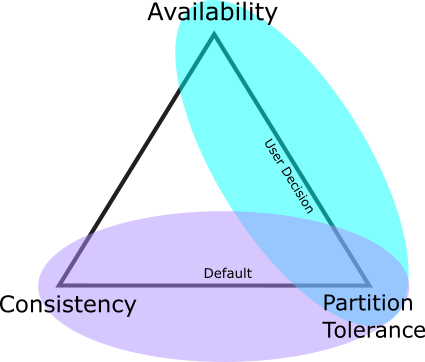
\includegraphics{img/rethinkCapTheorem.png}
    \caption{Overview of the CAP Theorem in RethinkDB}
    \label{fig:rethink_cap_theorem}
\end{figure}

\subsubsection{Performance}

In a test conducted by the RethinkDB core team the developers concluded that the database scales horizontally in a near linear fashion \autocite{rethinkdb:performance} as can be seen in \autoref{fig:rethink_rethink_performance}. The developers further imply that there will be ongoing efforts to improve upon this results.

\begin{figure}[ht]
    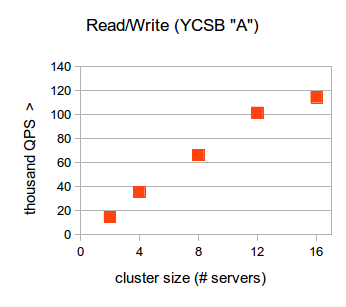
\includegraphics[width=.45\linewidth]{img/rethinkperf_rw.png} \quad
    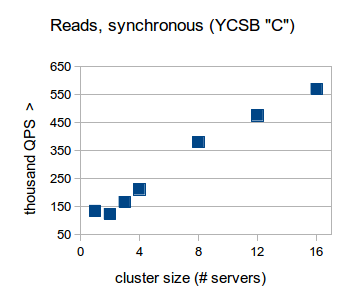
\includegraphics[width=0.45\linewidth]{img/rethinkperf_rsync.png}
    \\[\baselineskip]
    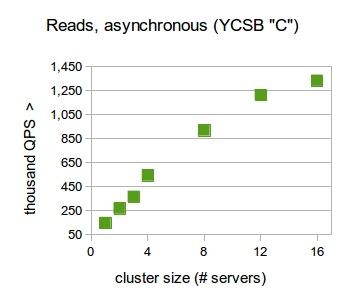
\includegraphics[width=0.45\linewidth]{img/rethinkperf_rasync.png} \quad
    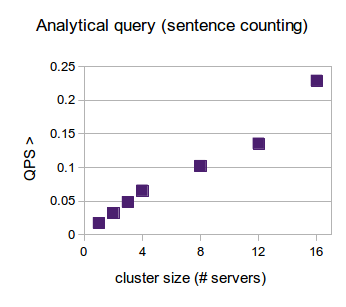
\includegraphics[width=0.45\linewidth]{img/rethinkperf_aquery.png}
    \caption{Overview of performance test results\autocite{rethinkdb:performance}}
    \label{fig:rethink_rethink_performance}
\end{figure}

\subsubsection{Comparison to real-time sync APIs}
The functionality of RethinkDB can be compared to many real-time sync API services like Pusher\footnote{https://pusher.com} or Firebase\footnote{https://firebase.google.com/products/realtime-database/}. There are some key differences between those kinds of systems and RethinkDB.

The capability to store information is the most noticeable difference. Sync APIs don't store any data. They are intended to send uniform event streams to a large amount of recipients. Other key differences can be taken from \autoref{tbl:rethink_realtimesync}.

\begin{table}[ht]
\caption{Comparison of RethinkDB and real-time sync APIs}
\label{tbl:rethink_realtimesync}
\centering
\begin{tabular}{|p{0.55\textwidth}|p{0.34\textwidth}|}
\hline
RethinkDB & Real-time sync APIs \\ \hline
Open source 
\newline
$\rightarrow$ Can be deployed on any infrastructure
&
Cloud Service \\ \hline
General Purpose Database System \newline
$\rightarrow$ Can run complex queries
&
Syncing documents
$\rightarrow$ limited querying\\ \hline
Designed to be accessed from an application server\newline
$\rightarrow$ More complex to set up \newline
$\rightarrow$ More flexible \newline
$\rightarrow$ Works for sophisticated applications
&
Access directly over browser \newline
$\rightarrow$ Easy to setup \newline
$\rightarrow$ Limits flexibility\\
\hline
\end{tabular}
\end{table}

\subsubsection{Use Cases}
RethinkDB is useful in any situation where data needs to be stored and distributed at the same time\autocite{rethinkdb:faq}. The following list contains major use cases for the database.

\begin{itemize}
    \item Collaborative web and mobile apps
    \item Streaming analytics apps
    \item Multiplayer games
    \item Real-time marketplaces
    \item Connected devices
\end{itemize}
There are some use cases RethinkDB should not be applied to, gathered in the following list.

\begin{itemize}
    \item Applications that need full ACID support
    \item Strong schema enforcement is required
    \item Computationally intensive analytics
    \item High write availability is critical
\end{itemize}

\subsubsection{Conclusion}

Working with RethinkDB we found the documentation to be extraordinarily comprehensive. Every major feature could be found described in great detail and supported by multiple examples. Nevertheless there is some confusion concerning the term of real-time databases, since many different definitions exist. This made it harder to evaluate the topic in general and specifically in connection with RethinkDB. This was complicated even further by the fact that RethinkDB in fact 'rethought' databases, delivering a product that can hardly be forced into predefined categories.

However, due to this impossibility to classify the database, RethinkDB was very refreshing to work with, providing many new features and combining the advantages of multiple different database types.

Working with the Database proved to be very convenient. The documentation made it easy to get used to the specifics of RethinkDB. We had no chance to use all the features ReQL gives the user, due to it having to many and specialised features. We also were not able to test the software in a cluster configuration. Therefore testing the behaviour with sharding and replication setting applied was not possible.

In general we found RethinkDB very useful and where able to identify fitting use cases while testing the database.

We think that not only real-time databases but also RethinkDB will become more and more important in the near future, with big data and IoT redefining the world of databases. 

\input{content/5_0_graph_db}


\printbibliography

\appendix
%!TEX root = ../main.tex

\chapter{Cassandra query example}\label{appendix:cassandra:queryExample}
\begin{verbatim}
Create database, table, insert and select data

CREATE KEYSPACE people
    WITH REPLICATION =
      { 'class' : 'SimpleStrategy', 'replication_factor' : 3 };
USE people;

CREATE COLUMNFAMILY users (
    username varchar PRIMARY KEY,
    name varchar,
    lastname varchar,
    email varchar,
    age int
);

INSERT INTO users (username, name, lastname, email)
    VALUES ('john', 'John', 'Smith', 'john@gmail.com');
INSERT INTO users (username, name, lastname, age)
    VALUES ('jack', 'Jack', 'Sparrow', 33);
INSERT INTO users (username, name, lastname, email, age)
    VALUES ('kate', 'Kate', 'Austen', null, 25);

SELECT * FROM users;

 username | age  | email          | lastname | name
----------+------+----------------+----------+------
     kate |   25 |           null |   Austen | Kate
     john | null | john@gmail.com |    Smith | John
     jack |   33 |           null |  Sparrow | Jack

$ nodetool flush

$ sstabletump /var/lib/cassandra/data/people/*/mc-1-big-Data.db
[
  {
    "partition" : {
      "key" : [ "kate" ],
      "position" : 0
    },
    "rows" : [
      {
        "type" : "row",
        "position" : 45,
        "liveness_info" : { "tstamp" : "2019-04-14T16:21:05.014317Z" },
        "cells" : [
          { "name" : "age", "value" : 25 },
          {
            "name" : "email",
            "deletion_info" :
              { "local_delete_time" : "2019-04-14T16:21:05Z" }
          },
          { "name" : "lastname", "value" : "Austen" },
          { "name" : "name", "value" : "Kate" }
        ]
      }
    ]
  },
  {
    "partition" : {
      "key" : [ "john" ],
      "position" : 46
    },
    "rows" : [
      {
        "type" : "row",
        "position" : 98,
        "liveness_info" : { "tstamp" : "2019-04-14T16:21:04.982207Z" },
        "cells" : [
          { "name" : "email", "value" : "john@gmail.com" },
          { "name" : "lastname", "value" : "Smith" },
          { "name" : "name", "value" : "John" }
        ]
      }
    ]
  },
  {
    "partition" : {
      "key" : [ "jack" ],
      "position" : 99
    },
    "rows" : [
      {
        "type" : "row",
        "position" : 144,
        "liveness_info" : { "tstamp" : "2019-04-14T16:21:05.002672Z" },
        "cells" : [
          { "name" : "age", "value" : 33 },
          { "name" : "lastname", "value" : "Sparrow" },
          { "name" : "name", "value" : "Jack" }
        ]
      }
    ]
  }
]
\end{verbatim}

\chapter[RethinkDB List of Drivers]{RethinkDB List of Drivers\footnote{https://www.rethinkdb.com/docs/install-drivers/}}\label{appendix:rethinkdb:listofdrivers}
\paragraph{Official Drivers}

\begin{itemize}
    \itemsep0em
    \item JavaScript
    \item Ruby
    \item Python
    \item Java
\end{itemize}

\paragraph{Community Drivers}

\begin{itemize}
    \itemsep0em
    \item C\#
    \item C++
    \item Clojure
    \item Common Lisp
    \item Dart
    \item Delphi
    \item Elixir
    \item Erlang
    \item Go
    \item Haskell
    \item Lua
    \item Nim
    \item Perl
    \item PHP
    \item R
    \item Rust
    \item Swift
\end{itemize}

\paragraph{Limited Drivers}

\begin{itemize}
    \itemsep0em
    \item Objective C
    \item Scala
\end{itemize}


\end{document}
